\documentclass[12pt]{report}
\usepackage{fullpage,graphicx,psfrag,amsmath,amsfonts,verbatim}
\usepackage[small,bf]{caption}
\usepackage{amsthm}
\usepackage{hyperref}
\usepackage{bbm} % for the indicator function to look good
\usepackage{color}
\usepackage{mathtools}
\usepackage{fancyhdr} % for the header
\usepackage{subcaption} % for subfigure
\usepackage{booktabs} % for toprule, midrule, bottomrule
\usepackage{adjustbox}
\input newcommand.tex
\setlength{\parindent}{0pt} % remove the automatic indentation

% \bibliographystyle{alpha}

\title{Preliminaries \vskip1cm 
\includegraphics{../../Figures/ihaveaquestion.jpg}}
\author{Fu Zixuan\thanks{Last compiled on \today}}
\date{}

\begin{document}
\maketitle

\newpage
\tableofcontents
\newpage
% \chapter{Year 2016-2019}
% \section{Descriptive Statistics}
\subsection{Stays per labor input}
% latex table generated in R 4.2.1 by xtable 1.8-4 package
% Mon May 13 09:35:12 2024
\begin{table}[ht]
\centering
\begin{tabular}{rlrrrrr}
  \hline
 & STJR\_LABEL & PUB & PLU & PNL & CHU & All \\ 
  \hline
1 & Q1 & 51.37 & 133.48 & 60.76 & 70.54 & 71.12 \\ 
  2 & Q2 & 105.17 & 181.73 & 98.77 & 99.00 & 124.31 \\ 
  3 & Q3 & 141.30 & 231.18 & 155.14 & 128.60 & 175.32 \\ 
  4 & Mean & 106.16 & 194.39 & 128.23 & 103.76 & 137.71 \\ 
  5 & Nobs & 2726.00 & 2004.00 & 741.00 & 606.00 & 6077.00 \\ 
   \hline
\end{tabular}
\caption{SJMD MCO} 
\end{table}

% latex table generated in R 4.2.1 by xtable 1.8-4 package
% Mon May 13 09:35:12 2024
\begin{table}[ht]
\centering
\begin{tabular}{rlrrrrr}
  \hline
 & STJR\_LABEL & PUB & PLU & PNL & CHU & All \\ 
  \hline
1 & Q1 & 208.36 & 181.51 & 177.67 & 500.10 & 198.23 \\ 
  2 & Q2 & 1036.97 & 272.76 & 491.50 & 847.58 & 493.31 \\ 
  3 & Q3 & 1427.00 & 430.11 & 1220.56 & 1154.48 & 1180.57 \\ 
  4 & Mean & 977.18 & 391.45 & 734.43 & 914.89 & 748.21 \\ 
  5 & Nobs & 2726.00 & 2004.00 & 741.00 & 606.00 & 6077.00 \\ 
   \hline
\end{tabular}
\caption{SJMD TOT} 
\end{table}

\clearpage
% latex table generated in R 4.2.1 by xtable 1.8-4 package
% Mon May 13 09:35:12 2024
\begin{table}[ht]
\centering
\begin{tabular}{rlrrrrr}
  \hline
 & STJR\_LABEL & PUB & PLU & PNL & CHU & All \\ 
  \hline
1 & Q1 & 23.80 & 138.27 & 32.23 & 33.15 & 35.41 \\ 
  2 & Q2 & 47.15 & 185.18 & 62.83 & 48.93 & 61.51 \\ 
  3 & Q3 & 62.56 & 240.04 & 108.09 & 57.38 & 150.86 \\ 
  4 & Mean & 47.11 & 214.42 & 93.66 & 46.43 & 108.00 \\ 
  5 & Nobs & 2736.00 & 2010.00 & 730.00 & 599.00 & 6075.00 \\ 
   \hline
\end{tabular}
\caption{SJINF MCO} 
\end{table}


% latex table generated in R 4.2.1 by xtable 1.8-4 package
% Mon May 13 09:35:12 2024
\begin{table}[ht]
\centering
\begin{tabular}{rlrrrrr}
  \hline
 & STJR\_LABEL & PUB & PLU & PNL & CHU & All \\ 
  \hline
1 & Q1 & 70.69 & 210.23 & 105.91 & 191.63 & 167.56 \\ 
  2 & Q2 & 476.89 & 284.89 & 304.42 & 434.84 & 347.90 \\ 
  3 & Q3 & 639.75 & 422.14 & 754.52 & 571.29 & 587.61 \\ 
  4 & Mean & 444.58 & 361.79 & 542.56 & 436.39 & 428.15 \\ 
  5 & Nobs & 2736.00 & 2010.00 & 730.00 & 599.00 & 6075.00 \\ 
   \hline
\end{tabular}
\caption{SJINF TOT} 
\end{table}

\clearpage
% latex table generated in R 4.2.1 by xtable 1.8-4 package
% Mon May 13 09:35:12 2024
\begin{table}[ht]
\centering
\begin{tabular}{rlrrrrr}
  \hline
 & STJR\_LABEL & PUB & PLU & PNL & CHU & All \\ 
  \hline
1 & Q1 & 17.37 & 233.39 & 27.01 & 31.97 & 32.09 \\ 
  2 & Q2 & 50.88 & 340.07 & 104.34 & 62.98 & 79.42 \\ 
  3 & Q3 & 76.24 & 487.77 & 198.55 & 82.86 & 257.67 \\ 
  4 & Mean & 53.11 & 472.98 & 152.45 & 63.58 & 204.27 \\ 
  5 & Nobs & 2730.00 & 1990.00 & 727.00 & 600.00 & 6047.00 \\ 
   \hline
\end{tabular}
\caption{SJAS MCO} 
\end{table}


% latex table generated in R 4.2.1 by xtable 1.8-4 package
% Mon May 13 09:35:12 2024
\begin{table}[ht]
\centering
\begin{tabular}{rlrrrrr}
  \hline
 & STJR\_LABEL & PUB & PLU & PNL & CHU & All \\ 
  \hline
1 & Q1 & 55.09 & 366.80 & 96.77 & 186.98 & 211.10 \\ 
  2 & Q2 & 508.07 & 535.53 & 464.22 & 582.30 & 529.11 \\ 
  3 & Q3 & 777.93 & 848.29 & 1262.24 & 826.61 & 827.01 \\ 
  4 & Mean & 525.48 & 828.41 & 929.30 & 583.77 & 679.50 \\ 
  5 & Nobs & 2730.00 & 1990.00 & 727.00 & 600.00 & 6047.00 \\ 
   \hline
\end{tabular}
\caption{SJAS TOT} 
\end{table}

\clearpage
\subsection{Share of outpatient stays}
\begin{figure}[!htb]
    \centering
    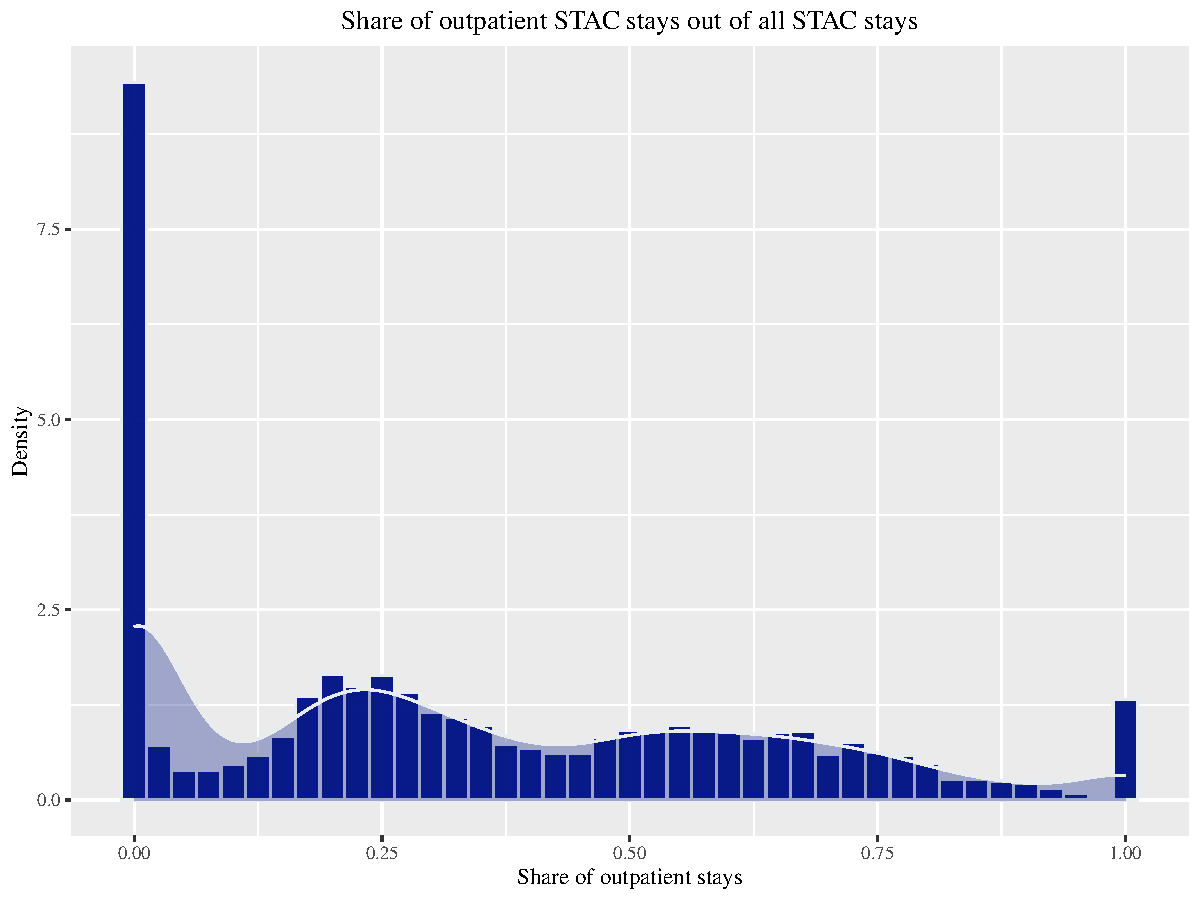
\includegraphics[width=0.8\textwidth]{../../Figures/2016-2019/STAC_share_pool.pdf}
\end{figure}

\clearpage
\begin{figure}[!htb]
    \centering
    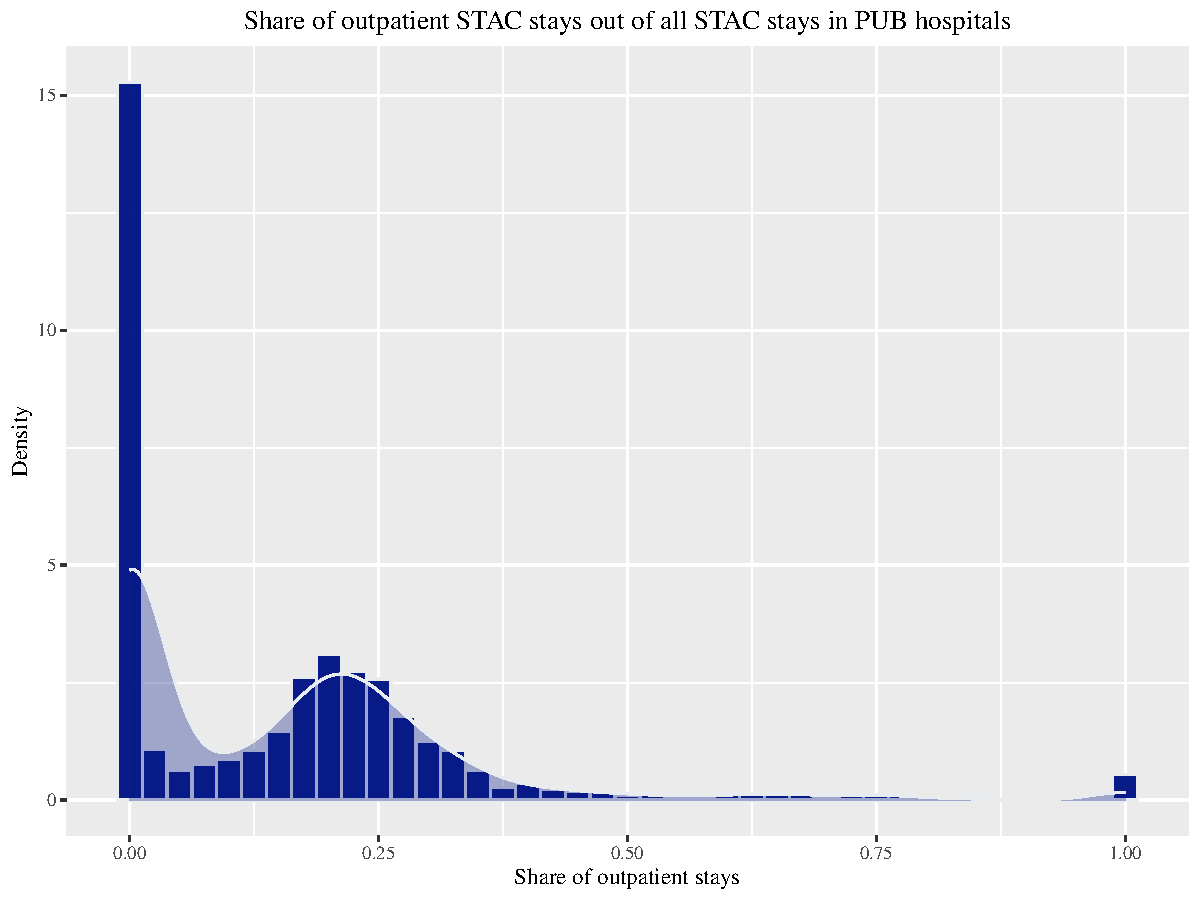
\includegraphics[width=0.8\textwidth]{../../Figures/2016-2019/STAC_share_PUB.pdf}
\end{figure}

\begin{figure}[!htb]
    \centering
    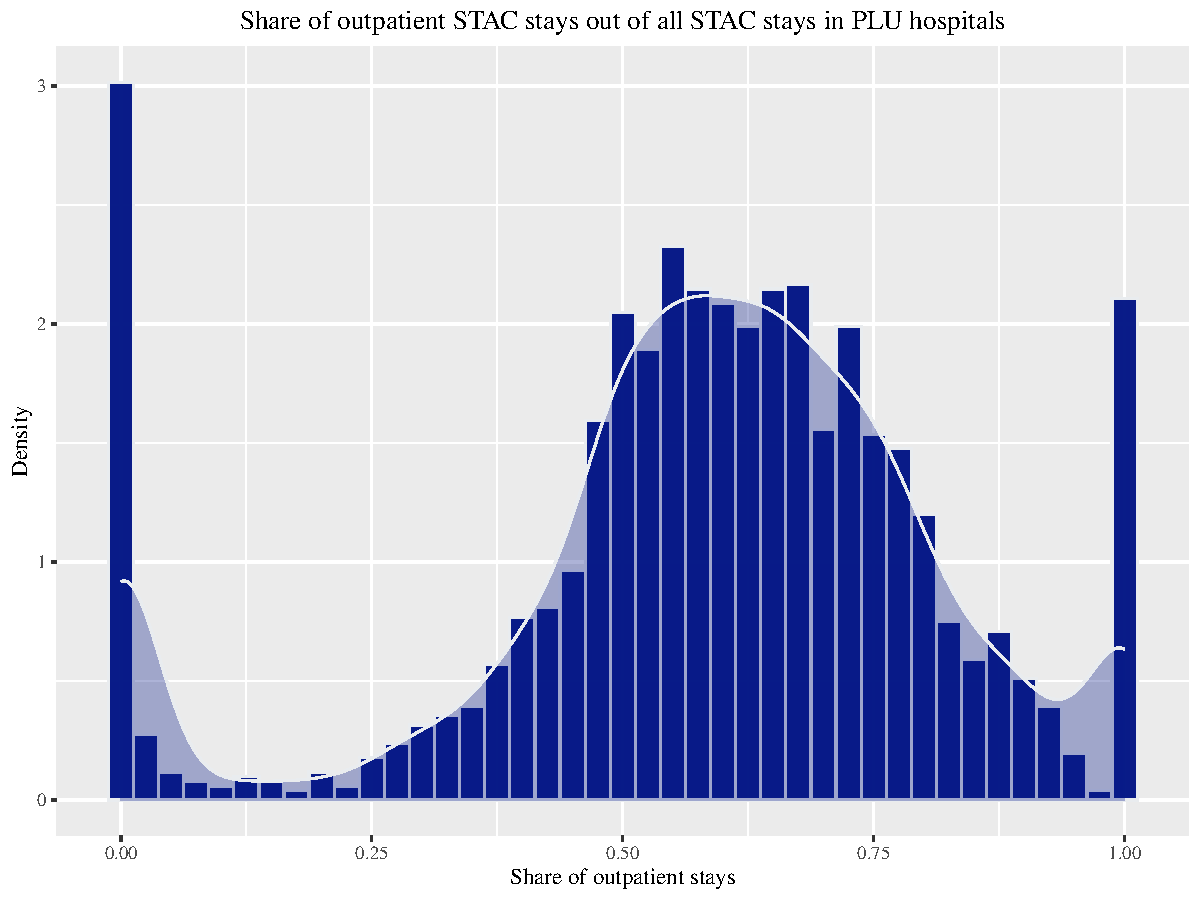
\includegraphics[width=0.8\textwidth]{../../Figures/2016-2019/STAC_share_PLU.pdf}
\end{figure}

\clearpage
\begin{figure}[!htb]
    \centering
    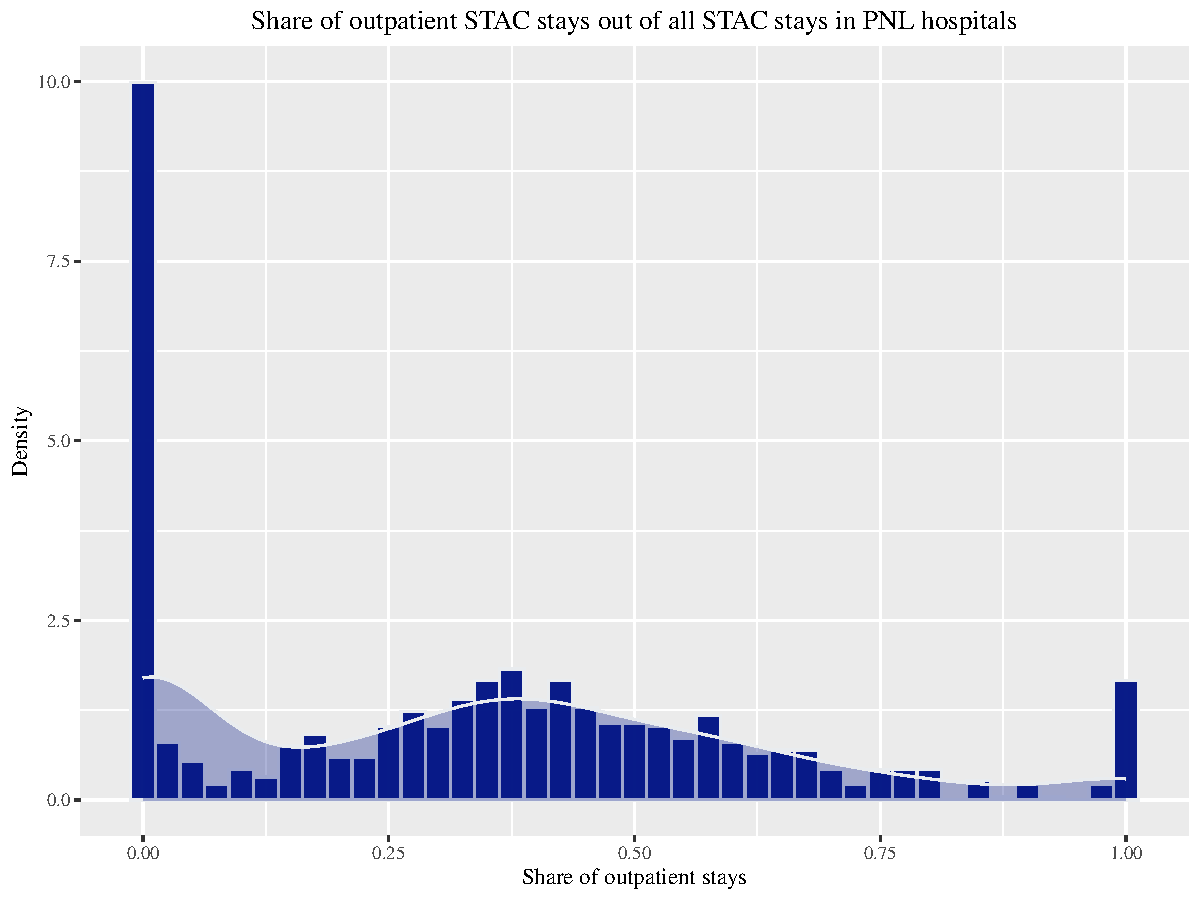
\includegraphics[width=0.8\textwidth]{../../Figures/2016-2019/STAC_share_PNL.pdf}
\end{figure}

\begin{figure}[!htb]
    \centering
    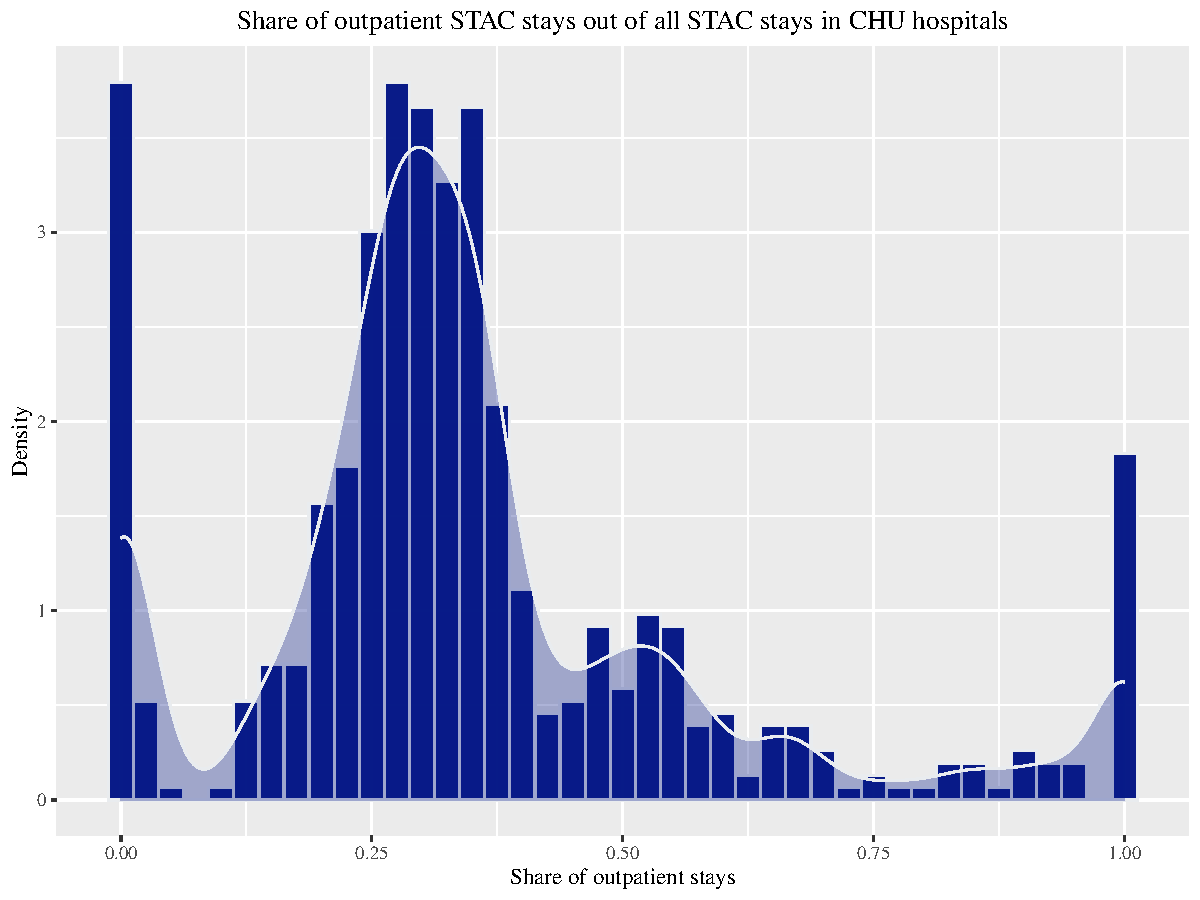
\includegraphics[width=0.8\textwidth]{../../Figures/2016-2019/STAC_share_CHU.pdf}
\end{figure}

\clearpage
\begin{figure}[!htb]
    \centering
    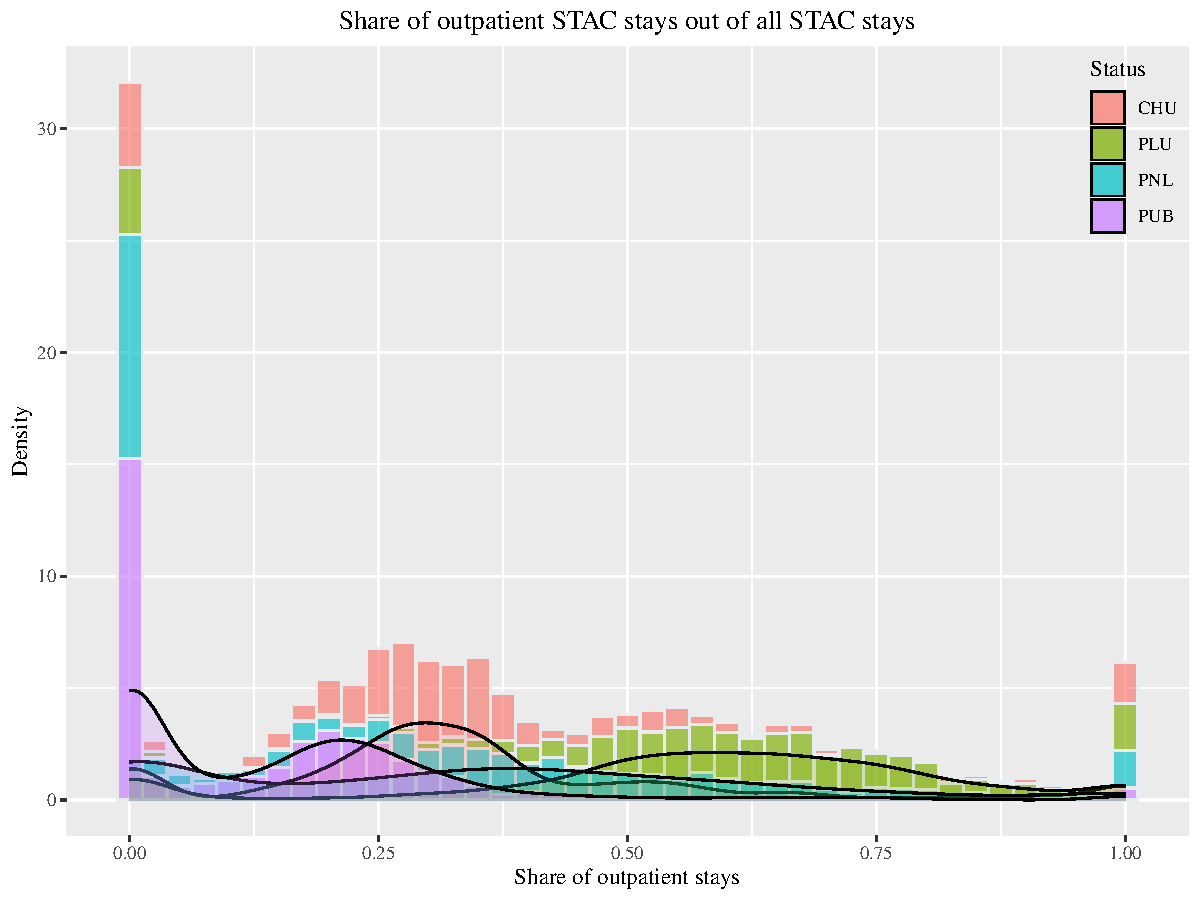
\includegraphics[width=0.8\textwidth]{../../Figures/2016-2019/STAC_share_all.pdf}
\end{figure}
\clearpage
\subsection{Average length of stay}
% latex table generated in R 4.2.1 by xtable 1.8-4 package
% Fri May 10 23:25:44 2024
\begin{table}[ht]
\centering
\begin{tabular}{rlrrrrr}
  \hline
 & STJR\_LABEL & PUB & PLU & PNL & CHU & All \\ 
  \hline
1 & Q1 & 5.12 & 3.13 & 4.22 & 5.05 & 4.05 \\ 
  2 & Q2 & 6.21 & 3.78 & 5.46 & 6.03 & 5.26 \\ 
  3 & Q3 & 11.83 & 4.53 & 10.08 & 8.60 & 8.47 \\ 
  4 & Mean & 8.76 & 4.18 & 7.53 & 7.42 & 6.99 \\ 
  5 & Std\_dev & 5.25 & 2.38 & 5.03 & 4.00 & 4.81 \\ 
  6 & Nobs & 2712.00 & 1926.00 & 715.00 & 584.00 & 5937.00 \\ 
   \hline
\end{tabular}
\end{table}


\begin{figure}[!htb]
    \centering
    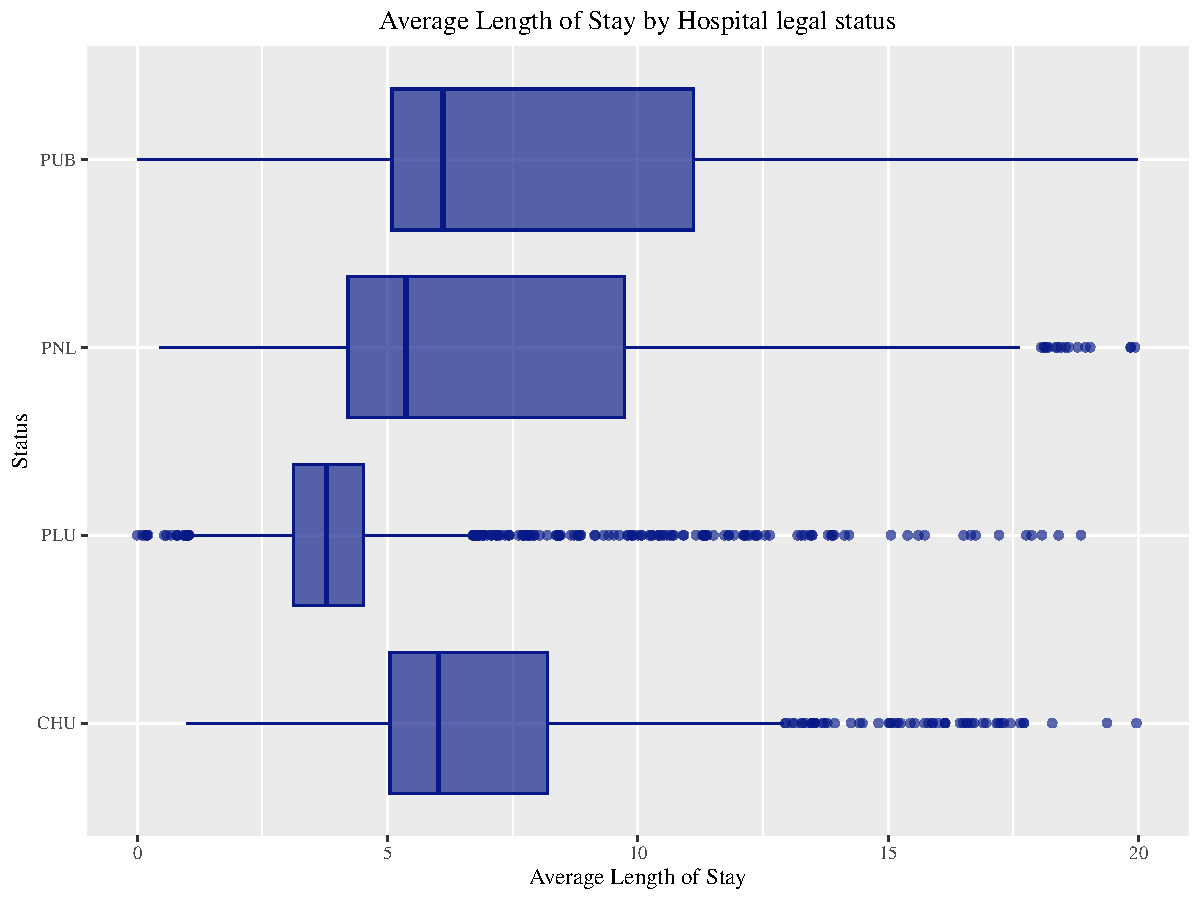
\includegraphics[width=0.8\textwidth]{../../Figures/2016-2019/ALOS.pdf}
\end{figure}
\clearpage
\subsection{Selection of patients}

% latex table generated in R 4.2.1 by xtable 1.8-4 package
% Mon May 13 09:36:57 2024
\begin{table}[ht]
\centering
\begin{tabular}{rlrrrr}
  \hline
 & size & CHU & PLU & PNL & PUB \\ 
  \hline
1 & 1 & 11.98 & 14.83 & 28.85 & 34.39 \\ 
  2 & 2 & 11.82 & 4.73 & 20.17 & 23.72 \\ 
  3 & 3 & 11.60 & 3.59 & 11.72 & 14.77 \\ 
  4 & 4 & 11.53 & 4.56 & 10.69 & 13.96 \\ 
   \hline
\end{tabular}
\caption{Average casemix index by hospital legal status and size of hospital} 
\end{table}


% \input{tex/reg_2016_2019.tex}

\chapter{Year 2016-2022}
\newpage
\section{Regression tables}

\subsection{WG, BG, Random effect, Correalted random effect(Mundlak)}
\paragraph{Notation}
\begin{itemize}
    \item Dependent variable: \begin{equation*}
              \underbrace{y}_{NT\times 1}= \begin{pmatrix}
                  y_1    \\
                  \vdots \\
                  y_N
              \end{pmatrix} \quad
              \underbrace{y_i}_{T\times 1} = \begin{pmatrix}
                  y_{i1} \\
                  \vdots \\
                  y_{iT}
              \end{pmatrix}
          \end{equation*}
    \item Independent variable:\begin{equation*}
              \underbrace{X}_{NT\times K}= \begin{pmatrix}
                  x_1    \\
                  \vdots \\
                  x_N
              \end{pmatrix} \quad
              \underbrace{x_i}_{T\times K} = \begin{pmatrix}
                  x_{i1} \\
                  \vdots \\
                  x_{iT}
              \end{pmatrix}
          \end{equation*}
    \item Matrix to calcualte the mean: \begin{equation*}
              B_T= d_T(d_T' d_T)^{-1}d_T'\quad \text{where} \quad d_T=\begin{pmatrix}
                  1 \\ \vdots \\ 1 \end{pmatrix}
          \end{equation*}
          Thus \begin{equation*}
              B_T y_1 = \begin{pmatrix}
                  \bar{y}_1 \\ \vdots \\ \bar{y}_1
              \end{pmatrix}
          \end{equation*}
          we set $B=I_N\otimes B_T$
    \item Matrix to demean the variable: \begin{equation*}
              W_T= I_T-B_T
          \end{equation*}
          Thus, \begin{equation*}
              W_T y_i = \begin{pmatrix}
                  y_{i1}-\bar{y}_1 \\ \vdots \\ y_{iT}-\bar{y}_1
              \end{pmatrix}
          \end{equation*}
          we set $W=I_N\otimes W_T$

\end{itemize}
\paragraph{Estimators}
\begin{itemize}
    \item WG: \begin{equation*}
              \hat{\beta}_{WG}=(X'WX)^{-1}X'W y
          \end{equation*}
    \item BG: \begin{equation*}
              \hat{\beta}_{BG}=(X'B X)^{-1}X'By\end{equation*}
    \item RE: A linear combination of WG and BG
    \item CRE (Mundlak): equivalent to WG
          \begin{quote}
              In empirical analysis of data consisting of repeated observations on economic units (time series on a cross section) it is often assumed that the coefficients of the quantitiative variables (slopes) are the same, whereas the coefficients of the qualitative variables (intercepts or effects) vary over units or periods. This is the constant-slope variable- intercept framework. In such an analysis an explicit account should be taken of the statistical dependence that exists between the quantitative variables and the effects. It is shown that when this is done, the random effect approach and the fixed effect approach yield the same estimate for the slopes, the "within" estimate. Any matrix combination of the "within" and "between" estimates is generally biased. When the "within" estimate is subject to a relatively large error a minimum mean square error can be applied, as is generally done in regression analysis. Such an estimator is developed here from a somewhat different point of departure.
          \end{quote}
\end{itemize}
% Denote $y=\text{ETP_INF}$, $x_1=\text{STAC INPATIENT}$, $x_2=\text{STAC
%         OUTPATIENT}$, $x_3=\text{SESSION}$\
\paragraph{Inference on $\theta_i$ and ($\beta$)}
If we apply the WG estimator $\hat{\beta}_{WG}= (X'WX)^{-1}X'W y$. The
estimated fixed effect is \begin{equation*}
    \begin{split}
        \hat{\theta}_i &= \frac{1}{T}\sum_{t=1}^T y_{it}-x_{it}\hat{\beta}_{WG}\\
        &= \frac{1}{T}\sum y_{it}-x_{it}\beta+\frac{1}{T}\sum x_{it}\beta-x_{it}\hat{\beta}_{WG}\\
        &= \theta_i+\frac{1}{T}\sum_t \epsilon_{it} + \frac{1}{T}\sum x_{it}(\beta-\hat{\beta}_{WG})\\
        & = \theta_i + \frac{1}{T}\sum_t \epsilon_{it} + \frac{1}{T}(X'WX)^{-1}X'W\epsilon \sum_t x_{it}\\
    \end{split}
\end{equation*}
It is clear that the second part follows a normal distribution $N(0, \sigma_i^2)$. The third part is where asymptotic kicks since \begin{equation*}
    \sqrt{N}\hat{\beta}_{WG} -\beta \sim N(0, \Sigma)
\end{equation*}

\paragraph{Recall the lectures...}
Assume a simple stripped down model where $y_{it}=\alpha_i+\epsilon_{it}$, two
cases \begin{enumerate}
    \item $y_{it}=\alpha_i+\epsilon_{it} \sim N(\alpha_i,\sigma^2)$
    \item $y_{it}=\alpha_i+\epsilon_{it} \sim N(\alpha_i,\sigma_i^2)$
\end{enumerate}
The estimator of $\alpha_i$ is \begin{equation*}
    \hat{\alpha}_i = \bar{y}_i
\end{equation*}

\paragraph{Estimate the $\sigma^2$ and $\sigma_i^2$}
The classical incidental parameter problem appears when we want to estimate
$\sigma^2$ or $\sigma_i^2$ because we only have an estimate of $\hat{\alpha}_i
    = \bar{y}_i$.
\begin{enumerate}
    \item $\sigma^2$: \begin{equation*}
              \hat{\sigma}^2 = \frac{1}{NT}\sum_{i=1}^N\sum_{t=1}^T (y_{it}-\hat{\alpha}_i)^2
          \end{equation*}
          \begin{itemize}
              \item The mean of the estimator is $\E\bra{\hat{\sigma}^2} = \sigma^2
                        (1-\frac{1}{T})$. Asymptotically \textbf{BIASED}. (Though We can deploy bias
                    correction techniques.)
              \item The variance of the estimator is $\Var\pa{\hat{\sigma}^2} =
                        \frac{2\sigma^4}{NT}(1-\frac{1}{T})$
          \end{itemize}
    \item $\sigma_i^2$: \begin{equation*}
              \hat{\sigma}_i^2 = \frac{1}{T}\sum_{t=1}^T (y_{it}-\hat{\alpha}_i)^2
          \end{equation*} This corresponds to the \textit{sufficient statistics} we will be talking about later.
\end{enumerate}
\paragraph{Estimate the variance of $\alpha$} If we treat $\alpha_i$ for each $i$
as a fixed number, and be agnostic about the possible latent distribution
$G_{\alpha}$ from which $\alpha_i$ is drawn from. We don't talk about the
variance of $\alpha$. Yet if we instead believe that all $\alpha_i$ are drawn
iidly from a distribution $G$, then it is interesting to estimate something
about $G$ (e.g. the moment of $\alpha$). \\ For example, we want to estimate
the \textbf{first moment} of $\alpha$ by \begin{equation*}
    \begin{split}
        \frac{1}{N}\sum \hat{\alpha}_i &= \frac{1}{N}\sum \alpha_i + \frac{1}{N}\sum \bar{\epsilon}_i\\
        \E\bra{\frac{1}{N}\sum \hat{\alpha}_i} &= \E\bra{\alpha_i} + 0
    \end{split}
\end{equation*}
This is unbiased.\\
Yet if we want to estimate the \textbf{second moment} of $\alpha$ by \begin{equation*}
    \begin{split}
        \frac{1}{N}\sum (\hat{\alpha}_i)^2 &= \frac{1}{N}\sum (\alpha_i+\bar{\epsilon}_i)^2\\
        &= \frac{1}{N}\sum \alpha_i^2 + \frac{1}{N}\sum \bar{\epsilon}_i^2 + \frac{2}{N}\sum \alpha_i\bar{\epsilon}_i\\
        \E\bra{\frac{1}{N}\sum (\hat{\alpha}_i)^2} &= \E\bra{\alpha_i^2} + \frac{1}{T}\sigma_i^2+0\\
    \end{split}
\end{equation*}
This is biased and the bias is $\frac{1}{T}\sigma_i^2$.

This is the issue we encountered when we go from the first moment of $\alpha$
to the second moment. It would be interesting to estimate the
$G_{\alpha}(\alpha_i)$ directly using non parametric convex optimization
methods.\\ Or when $\sigma_i^2$ is heterogeneous, it would be
(challenging/interesting) to estimate $H_{\alpha,\sigma}(\alpha_i,\sigma_i)$
directly.


% \newpage
\section{Regression tables}

\subsection{WG, BG, Random effect, Correalted random effect(Mundlak)}
\paragraph{Notation}
\begin{itemize}
    \item Dependent variable: \begin{equation*}
              \underbrace{y}_{NT\times 1}= \begin{pmatrix}
                  y_1    \\
                  \vdots \\
                  y_N
              \end{pmatrix} \quad
              \underbrace{y_i}_{T\times 1} = \begin{pmatrix}
                  y_{i1} \\
                  \vdots \\
                  y_{iT}
              \end{pmatrix}
          \end{equation*}
    \item Independent variable:\begin{equation*}
              \underbrace{X}_{NT\times K}= \begin{pmatrix}
                  x_1    \\
                  \vdots \\
                  x_N
              \end{pmatrix} \quad
              \underbrace{x_i}_{T\times K} = \begin{pmatrix}
                  x_{i1} \\
                  \vdots \\
                  x_{iT}
              \end{pmatrix}
          \end{equation*}
    \item Matrix to calcualte the mean: \begin{equation*}
              B_T= d_T(d_T' d_T)^{-1}d_T'\quad \text{where} \quad d_T=\begin{pmatrix}
                  1 \\ \vdots \\ 1 \end{pmatrix}
          \end{equation*}
          Thus \begin{equation*}
              B_T y_1 = \begin{pmatrix}
                  \bar{y}_1 \\ \vdots \\ \bar{y}_1
              \end{pmatrix}
          \end{equation*}
          we set $B=I_N\otimes B_T$
    \item Matrix to demean the variable: \begin{equation*}
              W_T= I_T-B_T
          \end{equation*}
          Thus, \begin{equation*}
              W_T y_i = \begin{pmatrix}
                  y_{i1}-\bar{y}_1 \\ \vdots \\ y_{iT}-\bar{y}_1
              \end{pmatrix}
          \end{equation*}
          we set $W=I_N\otimes W_T$

\end{itemize}
\paragraph{Estimators}
\begin{itemize}
    \item WG: \begin{equation*}
              \hat{\beta}_{WG}=(X'WX)^{-1}X'W y
          \end{equation*}
    \item BG: \begin{equation*}
              \hat{\beta}_{BG}=(X'B X)^{-1}X'By\end{equation*}
    \item RE: A linear combination of WG and BG
    \item CRE (Mundlak): equivalent to WG
          \begin{quote}
              In empirical analysis of data consisting of repeated observations on economic units (time series on a cross section) it is often assumed that the coefficients of the quantitiative variables (slopes) are the same, whereas the coefficients of the qualitative variables (intercepts or effects) vary over units or periods. This is the constant-slope variable- intercept framework. In such an analysis an explicit account should be taken of the statistical dependence that exists between the quantitative variables and the effects. It is shown that when this is done, the random effect approach and the fixed effect approach yield the same estimate for the slopes, the "within" estimate. Any matrix combination of the "within" and "between" estimates is generally biased. When the "within" estimate is subject to a relatively large error a minimum mean square error can be applied, as is generally done in regression analysis. Such an estimator is developed here from a somewhat different point of departure.
          \end{quote}
\end{itemize}
% Denote $y=\text{ETP_INF}$, $x_1=\text{STAC INPATIENT}$, $x_2=\text{STAC
%         OUTPATIENT}$, $x_3=\text{SESSION}$\
\paragraph{Inference on $\theta_i$ and ($\beta$)}
If we apply the WG estimator $\hat{\beta}_{WG}= (X'WX)^{-1}X'W y$. The
estimated fixed effect is \begin{equation*}
    \begin{split}
        \hat{\theta}_i &= \frac{1}{T}\sum_{t=1}^T y_{it}-x_{it}\hat{\beta}_{WG}\\
        &= \frac{1}{T}\sum y_{it}-x_{it}\beta+\frac{1}{T}\sum x_{it}\beta-x_{it}\hat{\beta}_{WG}\\
        &= \theta_i+\frac{1}{T}\sum_t \epsilon_{it} + \frac{1}{T}\sum x_{it}(\beta-\hat{\beta}_{WG})\\
        & = \theta_i + \frac{1}{T}\sum_t \epsilon_{it} + \frac{1}{T}(X'WX)^{-1}X'W\epsilon \sum_t x_{it}\\
    \end{split}

\end{equation*}
\begin{question}
    How to estimate the variance of $\hat{\theta}_i$? How to estimate the variance of $\alpah$?
\end{question}

\subsection{Specification}\hypertarget{home}{}
\paragraph{Model 1} (Pseudoc Poisson)
\begin{equation*}
    \begin{split}
        y_{it}&=x_{it1}^{\beta_1}x_{it2}^{\beta_2}x_{it3}^{\beta_3}\theta_i\epsilon_{it}\\
        &= f(x_{it};\beta)\theta_i\epsilon_{it}\\
    \end{split}
\end{equation*}

Tables: \hyperlink{reg_inf_pois_2022}{Pois}

\paragraph{Reference} to Koen Jochman's lecture notes on panel data and model with multiplicative
effect:
\begin{equation*}
    y_{it}=f(x_{it};\beta)\theta_i\epsilon_{it} \quad \text{where} \quad \E\bra{\epsilon_{it}|x_{i1},\ldots,x_{iT},\theta_i}=1
\end{equation*}
Then following the same logic in additive effect, we difference out individual effect to get:
\begin{equation*}
    \E\bra{\frac{y_{it}}{f(x_{it};\beta)}-\frac{y_{i,t-1}}{f(x_{i,t-1};\beta)}\bigg | x_{i1},\ldots,x_{iT}}=0
\end{equation*}
Similarly, \begin{equation*}
    \E\bra{\frac{y_{it}}{f(x_{it};\beta)}-\frac{\sum_{t=1}y_{it}}{\sum_{t=1}f(x_{it};\beta)}\bigg | x_{i1},\ldots,x_{iT}}=0
\end{equation*}
One of the unconditional moment equation given rise to is \begin{equation}
    \E\bra{x_it\pa{\frac{y_{it}}{f(x_{it};\beta)}-\frac{\sum_{t=1}y_{it}}{\sum_{t=1}f(x_{it};\beta)}}}=0
\end{equation}
The moment conditon is often called pseudo-poisson estimator (as if assuming $y_it|x_{i1},\ldots,x_{iT},\theta_i\sim Poisson(f(x_{it};\beta)\theta_i)$ and then use maximum likelihood.)
When regressors are not strictly exogenous, we can construct a \textbf{differencing} based estimator based on sequential moment restrictions.
The \verb+fixest+ package doesn't provide the differencing based estimator. \\
\textbf{TO BE CONSTRUCTED BY HAND LATER.}
\paragraph{Model 2} (OLS)
\begin{align*}
    \log(y_{it}) & =\log(x_{it1})\beta_1+\log(x_{it2})\beta_2+\log(x_{it3})\beta_3+\log(\theta_i)+\log(\epsilon_{it}) \\
\end{align*}
LHS: log(ETP INF); \\ RHS: log(STAC INPATIENT), log(STAC OUTPATIENT),
log(SESSION),CASEMIX
\\Table: \hyperlink{reg_inf_ols_2022}{OLS},
\hyperlink{reg_inf_lag_2022}{OLS\_lag1}
\\Figure: \hyperlink{FE_OLS_FI}{FixedEffect\_OLS}

\begin{remark}
    The Pseudo poisson and Log OLS are equivalent if we assume that $\epsilon_{it}$ is independent of $x_{it}$ and $\theta_i$.
\end{remark}

\begin{remark}
    The Mundlak (1978) approach is to include the average of the individual-specific variables $\bar{x_i}$ in the regression. He shows that it is equivalent to within group estimator.
    (Correlated random effect $\sim$ WG estimator). If the true model is \begin{equation*}
        y_{it}=x_{it}\beta+\theta_i+\epsilon_{it}
    \end{equation*} and $E(\theta_i|\bar{x}_i)=\bar{x}_i\gamma+\tilde{\theta}_i$, then
    \begin{equation*}
        y_{it}=(x_{it}-\bar{x}_i)\beta+\bar{x}_i(\gamma+\beta)+\tilde{\theta}_i+\epsilon_{it}
        (x_{it}-\bar{x}_i)\beta_1+\bar{x}_i\beta_2+\tilde{\theta}_i+\epsilon_{it}
    \end{equation*}
    Only when the $\theta_i$ is uncorrelated with $x_{it}$, the $\beta_1 = \beta_2$.
\end{remark}

\newpage
\hypertarget{reg_inf_pois_2022}{Pois}

\begingroup
\centering
\begin{tabular}{lcc}
   \tabularnewline \midrule \midrule
   Dependent Variable: & \multicolumn{2}{c}{ETP\_INF}\\
   Model:              & (1)         & (2)\\  
   \midrule
   \emph{Variables}\\
   log(SEJHC\_MCO)     & 0.158$^{a}$ & 0.727$^{a}$\\   
                       & (0.028)     & (0.026)\\   
   log(SEJHP\_MCO)     & 0.044$^{a}$ & 0.107$^{a}$\\   
                       & (0.011)     & (0.019)\\   
   log(SEANCES\_MED)   & 0.032$^{a}$ & 0.043$^{a}$\\   
                       & (0.008)     & (0.011)\\   
   CASEMIX             & 0.007$^{a}$ & 0.014$^{a}$\\   
                       & (0.002)     & (0.003)\\   
   \midrule
   \emph{Fixed-effects}\\
   FI                  & Yes         & \\  
   FI\_EJ              &             & Yes\\  
   \midrule
   \emph{Fit statistics}\\
   Observations        & 3,928       & 3,928\\  
   Squared Correlation & 0.995       & 0.983\\  
   Pseudo R$^2$        & 0.966       & 0.956\\  
   \midrule \midrule
   \multicolumn{3}{l}{\emph{Signif. Codes: a: 0.01, b: 0.05, c: 0.1}}\\
\end{tabular}
\par\endgroup



\hyperlink{home}{Back}
\bigskip

\newpage
\hypertarget{reg_inf_ols_2022}{OLS}

\begingroup
\centering
\begin{tabular}{lcc}
   \tabularnewline \midrule \midrule
   Dependent Variable: & \multicolumn{2}{c}{log(ETP\_INF)}\\
   Model:              & (1)         & (2)\\  
   \midrule
   \emph{Variables}\\
   log(SEJHC\_MCO)     & 0.184$^{a}$ & 0.676$^{a}$\\   
                       & (0.026)     & (0.031)\\   
   log(SEJHP\_MCO)     & 0.032$^{a}$ & 0.097$^{a}$\\   
                       & (0.011)     & (0.022)\\   
   log(SEANCES\_MED)   & 0.021$^{a}$ & 0.037$^{a}$\\   
                       & (0.006)     & (0.010)\\   
   CASEMIX             & 0.007$^{b}$ & 0.013$^{a}$\\   
                       & (0.003)     & (0.004)\\   
   \midrule
   \emph{Fixed-effects}\\
   FI                  & Yes         & \\  
   FI\_EJ              &             & Yes\\  
   \midrule
   \emph{Fit statistics}\\
   Observations        & 3,923       & 3,923\\  
   Squared Correlation & 0.993       & 0.980\\  
   Pseudo R$^2$        & 1.77        & 1.39\\  
   \midrule \midrule
   \multicolumn{3}{l}{\emph{Signif. Codes: a: 0.01, b: 0.05, c: 0.1}}\\
\end{tabular}
\par\endgroup



\hyperlink{home}{Back}
\bigskip
\newpage
\hypertarget{reg_inf_lag_2022}{OLS\_lag1}

\begingroup
\centering
\begin{tabular}{lcc}
   \tabularnewline \midrule \midrule
   Dependent Variable: & \multicolumn{2}{c}{log(ETP\_INF)}\\
   Model:              & (1)         & (2)\\  
   \midrule
   \emph{Variables}\\
   log(SEJHC\_MCO)     & 0.222$^{a}$ & 0.692$^{a}$\\   
                       & (0.049)     & (0.036)\\   
   log(SEJHP\_MCO)     & 0.093$^{a}$ & 0.111$^{a}$\\   
                       & (0.025)     & (0.032)\\   
   log(SEANCES\_MED)   & 0.040$^{c}$ & 0.047$^{a}$\\   
                       & (0.023)     & (0.015)\\   
   CASEMIX             & 0.013$^{a}$ & 0.014$^{a}$\\   
                       & (0.003)     & (0.005)\\   
   \midrule
   \emph{Fixed-effects}\\
   FI                  & Yes         & \\  
   FI\_EJ              &             & Yes\\  
   \midrule
   \emph{Fit statistics}\\
   Observations        & 3,151       & 3,151\\  
   Squared Correlation & 0.994       & 0.983\\  
   Pseudo R$^2$        & 1.84        & 1.48\\  
   \midrule \midrule
   \multicolumn{3}{l}{\emph{Signif. Codes: a: 0.01, b: 0.05, c: 0.1}}\\
\end{tabular}
\par\endgroup



\hyperlink{home}{Back}
\bigskip
\newpage
\hypertarget{FE_OLS_FI}{FixedEffect\_OLS} Fixed effects extracted from OLS regression with fixed effect on each FI (not FI\_EJ).
\begin{figure}[!htbp]
    \centering
    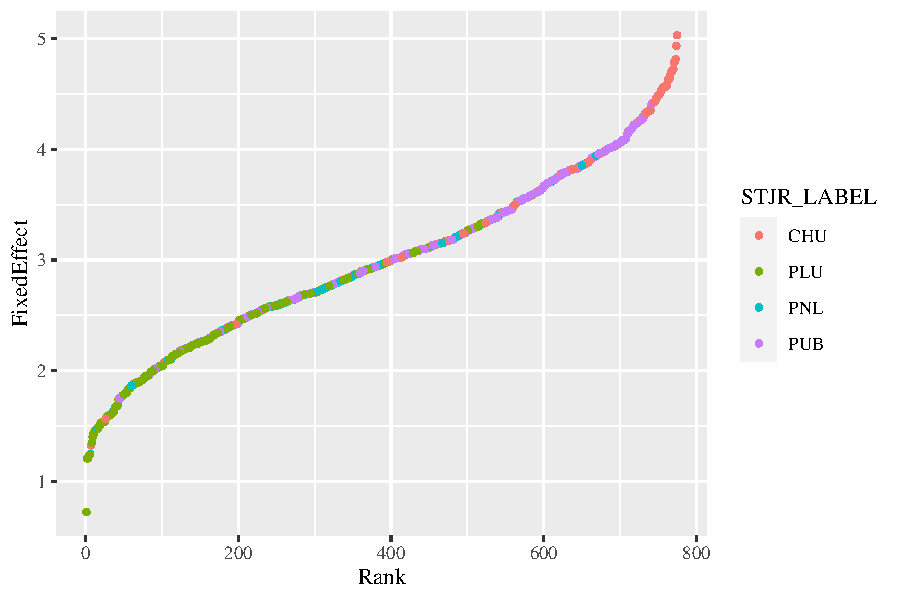
\includegraphics[width=0.8\textwidth]{../../Figures/2016-2022/FE_ols_FI.pdf}
    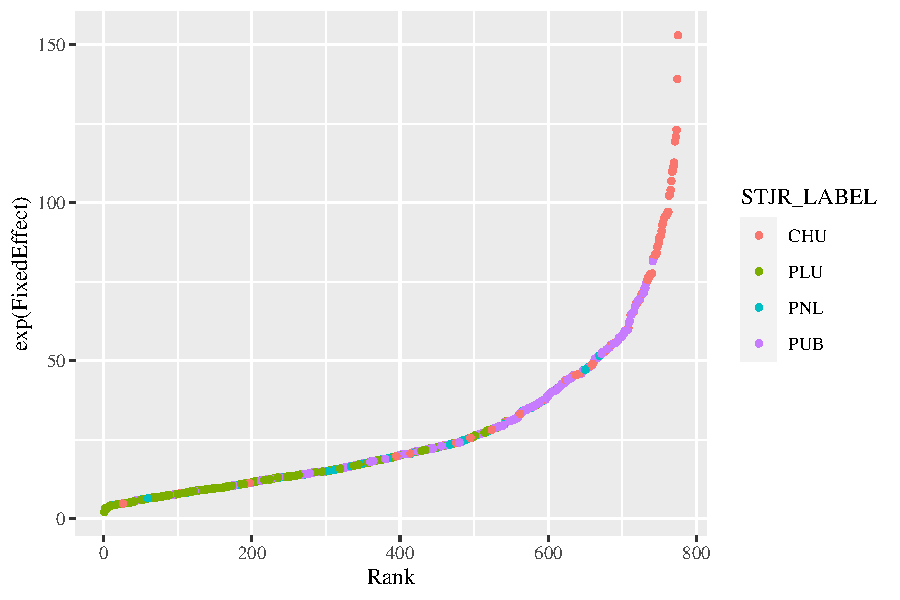
\includegraphics[width=0.8\textwidth]{../../Figures/2016-2022/FE_ols_FI_e.pdf}
\end{figure}
\hyperlink{home}{Back}
\bigskip
% \newpage
% \section{Descriptive Statistics}
\subsection{Stays per labor input}
% latex table generated in R 4.2.1 by xtable 1.8-4 package
% Mon May 13 09:40:49 2024
\begin{table}[ht]
\centering
\begin{tabular}{rlrrrrr}
  \hline
 & STJR\_LABEL & PUB & PLU & PNL & CHU & All \\ 
  \hline
1 & Q1 & 51.37 & 133.48 & 60.76 & 70.54 & 71.12 \\ 
  2 & Q2 & 105.17 & 181.73 & 98.77 & 99.00 & 124.31 \\ 
  3 & Q3 & 141.30 & 231.18 & 155.14 & 128.60 & 175.32 \\ 
  4 & Mean & 106.16 & 194.39 & 128.23 & 103.76 & 137.71 \\ 
  5 & Nobs & 2726.00 & 2004.00 & 741.00 & 606.00 & 6077.00 \\ 
   \hline
\end{tabular}
\caption{SJMD MCO} 
\end{table}

% latex table generated in R 4.2.1 by xtable 1.8-4 package
% Mon May 13 09:40:49 2024
\begin{table}[ht]
\centering
\begin{tabular}{rlrrrrr}
  \hline
 & STJR\_LABEL & PUB & PLU & PNL & CHU & All \\ 
  \hline
1 & Q1 & 208.36 & 181.51 & 177.67 & 500.10 & 198.23 \\ 
  2 & Q2 & 1036.97 & 272.76 & 491.50 & 847.58 & 493.31 \\ 
  3 & Q3 & 1427.00 & 430.11 & 1220.56 & 1154.48 & 1180.57 \\ 
  4 & Mean & 977.18 & 391.45 & 734.43 & 914.89 & 748.21 \\ 
  5 & Nobs & 2726.00 & 2004.00 & 741.00 & 606.00 & 6077.00 \\ 
   \hline
\end{tabular}
\caption{SJMD TOT} 
\end{table}


% latex table generated in R 4.2.1 by xtable 1.8-4 package
% Mon May 13 09:40:50 2024
\begin{table}[ht]
\centering
\begin{tabular}{rlrrrrr}
  \hline
 & STJR\_LABEL & PUB & PLU & PNL & CHU & All \\ 
  \hline
1 & Q1 & 23.80 & 138.27 & 32.23 & 33.15 & 35.41 \\ 
  2 & Q2 & 47.15 & 185.18 & 62.83 & 48.93 & 61.51 \\ 
  3 & Q3 & 62.56 & 240.04 & 108.09 & 57.38 & 150.86 \\ 
  4 & Mean & 47.11 & 214.42 & 93.66 & 46.43 & 108.00 \\ 
  5 & Nobs & 2736.00 & 2010.00 & 730.00 & 599.00 & 6075.00 \\ 
   \hline
\end{tabular}
\caption{SJINF MCO} 
\end{table}


% latex table generated in R 4.2.1 by xtable 1.8-4 package
% Mon May 13 09:40:50 2024
\begin{table}[ht]
\centering
\begin{tabular}{rlrrrrr}
  \hline
 & STJR\_LABEL & PUB & PLU & PNL & CHU & All \\ 
  \hline
1 & Q1 & 70.69 & 210.23 & 105.91 & 191.63 & 167.56 \\ 
  2 & Q2 & 476.89 & 284.89 & 304.42 & 434.84 & 347.90 \\ 
  3 & Q3 & 639.75 & 422.14 & 754.52 & 571.29 & 587.61 \\ 
  4 & Mean & 444.58 & 361.79 & 542.56 & 436.39 & 428.15 \\ 
  5 & Nobs & 2736.00 & 2010.00 & 730.00 & 599.00 & 6075.00 \\ 
   \hline
\end{tabular}
\caption{SJINF TOT} 
\end{table}


% latex table generated in R 4.2.1 by xtable 1.8-4 package
% Mon May 13 09:40:50 2024
\begin{table}[ht]
\centering
\begin{tabular}{rlrrrrr}
  \hline
 & STJR\_LABEL & PUB & PLU & PNL & CHU & All \\ 
  \hline
1 & Q1 & 17.37 & 233.39 & 27.01 & 31.97 & 32.09 \\ 
  2 & Q2 & 50.88 & 340.07 & 104.34 & 62.98 & 79.42 \\ 
  3 & Q3 & 76.24 & 487.77 & 198.55 & 82.86 & 257.67 \\ 
  4 & Mean & 53.11 & 472.98 & 152.45 & 63.58 & 204.27 \\ 
  5 & Nobs & 2730.00 & 1990.00 & 727.00 & 600.00 & 6047.00 \\ 
   \hline
\end{tabular}
\caption{SJAS MCO} 
\end{table}


% latex table generated in R 4.2.1 by xtable 1.8-4 package
% Mon May 13 09:40:50 2024
\begin{table}[ht]
\centering
\begin{tabular}{rlrrrrr}
  \hline
 & STJR\_LABEL & PUB & PLU & PNL & CHU & All \\ 
  \hline
1 & Q1 & 55.09 & 366.80 & 96.77 & 186.98 & 211.10 \\ 
  2 & Q2 & 508.07 & 535.53 & 464.22 & 582.30 & 529.11 \\ 
  3 & Q3 & 777.93 & 848.29 & 1262.24 & 826.61 & 827.01 \\ 
  4 & Mean & 525.48 & 828.41 & 929.30 & 583.77 & 679.50 \\ 
  5 & Nobs & 2730.00 & 1990.00 & 727.00 & 600.00 & 6047.00 \\ 
   \hline
\end{tabular}
\caption{SJAS TOT} 
\end{table}

\clearpage
\subsection{Share of outpatient stays}
\begin{figure}[!htb]
    \centering
    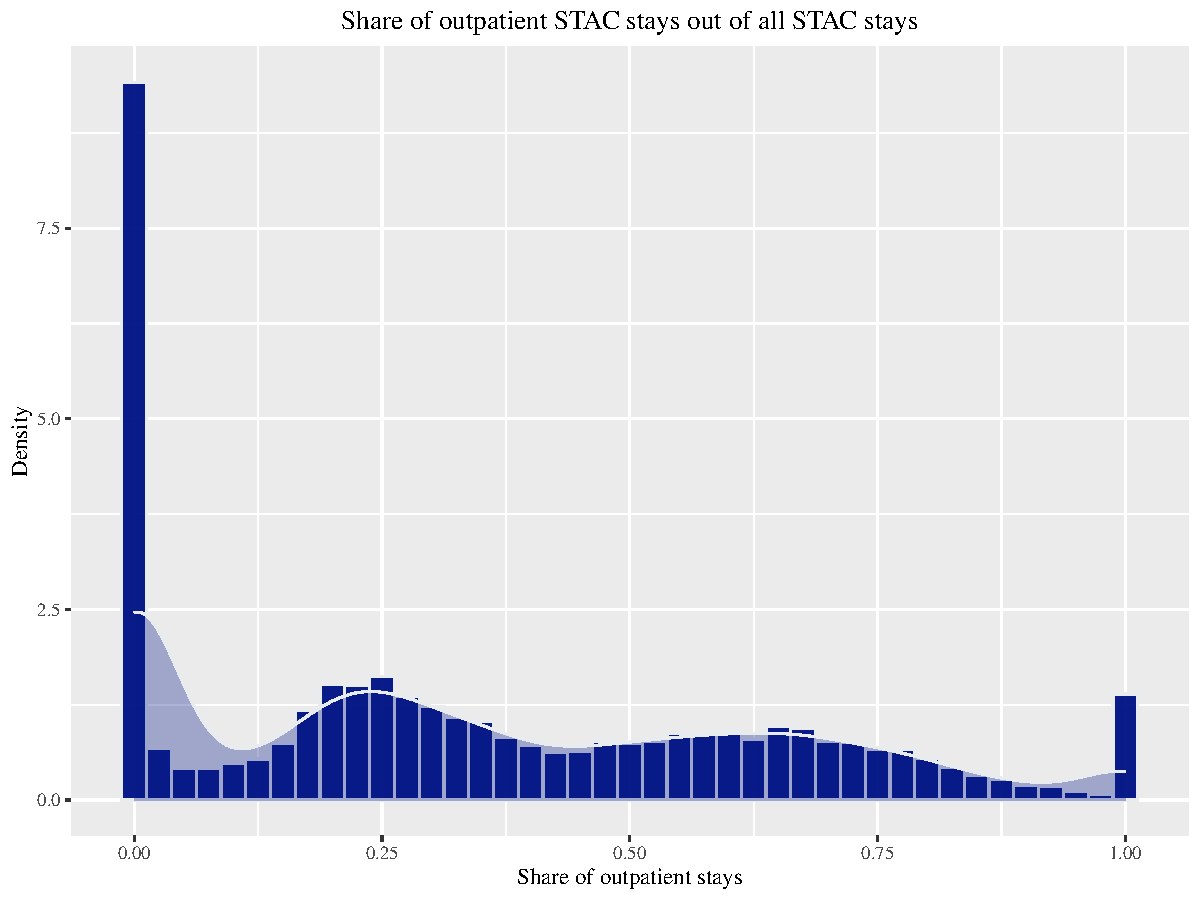
\includegraphics[width=0.8\textwidth]{../../Figures/2016-2022/STAC_share_pool.pdf}
\end{figure}

\bigskip
\begin{figure}[!htb]
    \centering
    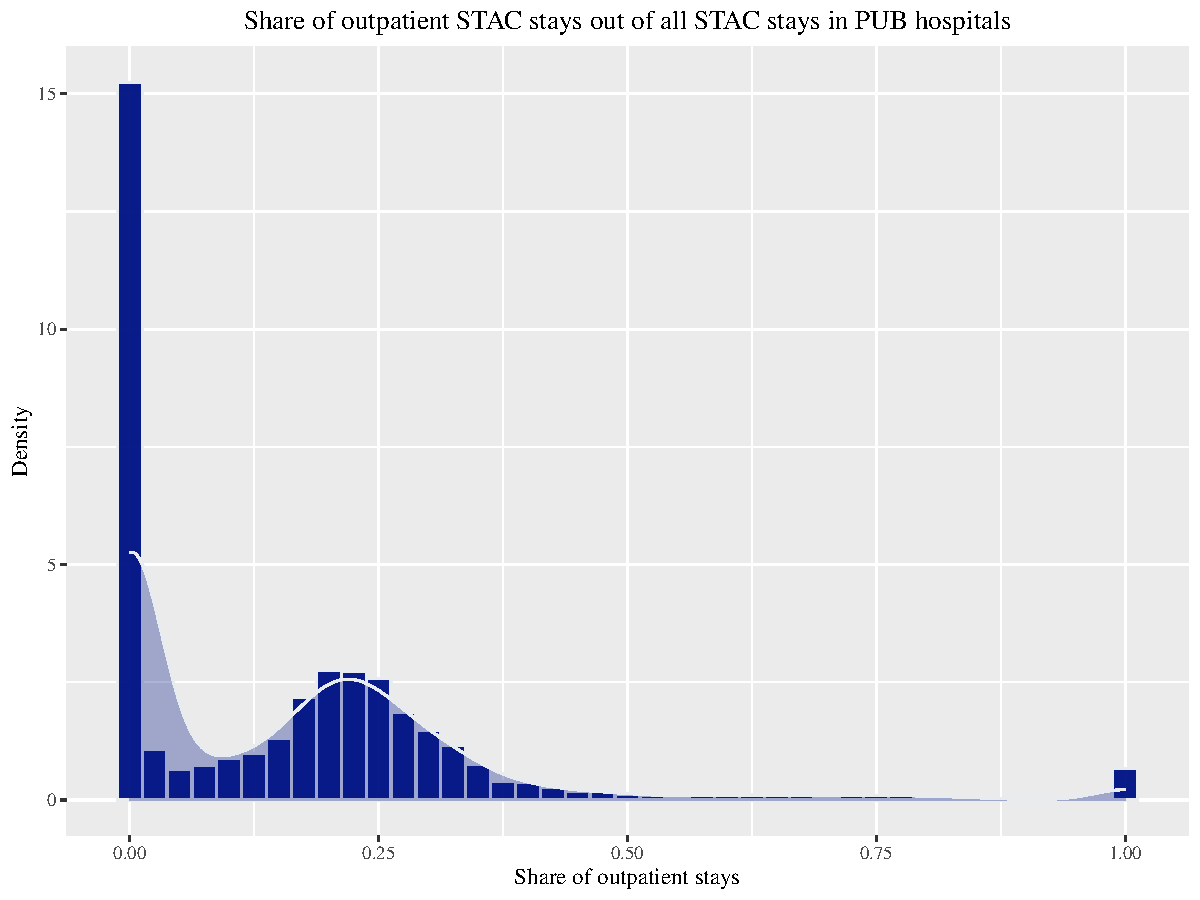
\includegraphics[width=0.8\textwidth]{../../Figures/2016-2022/STAC_share_PUB.pdf}
\end{figure}

\begin{figure}[!htb]
    \centering
    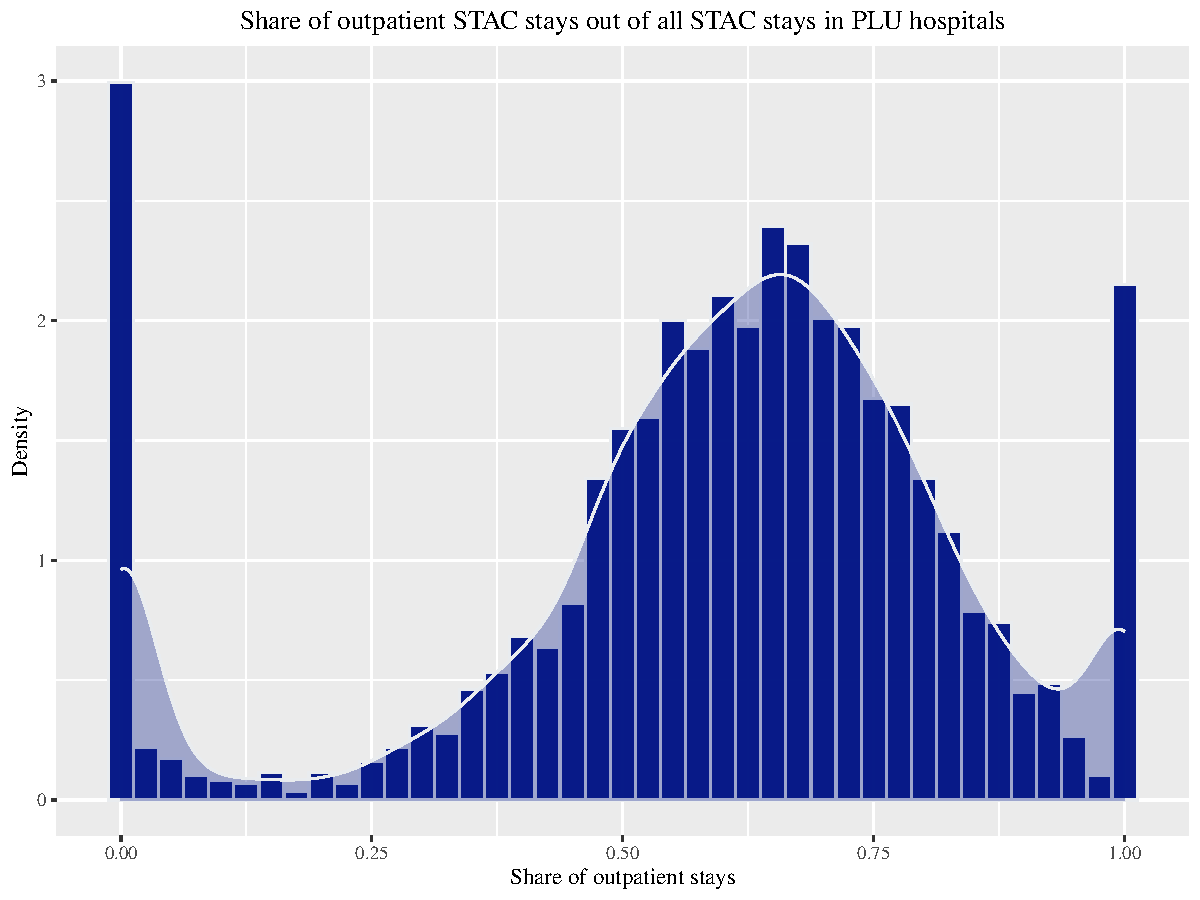
\includegraphics[width=0.8\textwidth]{../../Figures/2016-2022/STAC_share_PLU.pdf}
\end{figure}

\bigskip
\begin{figure}[!htb]
    \centering
    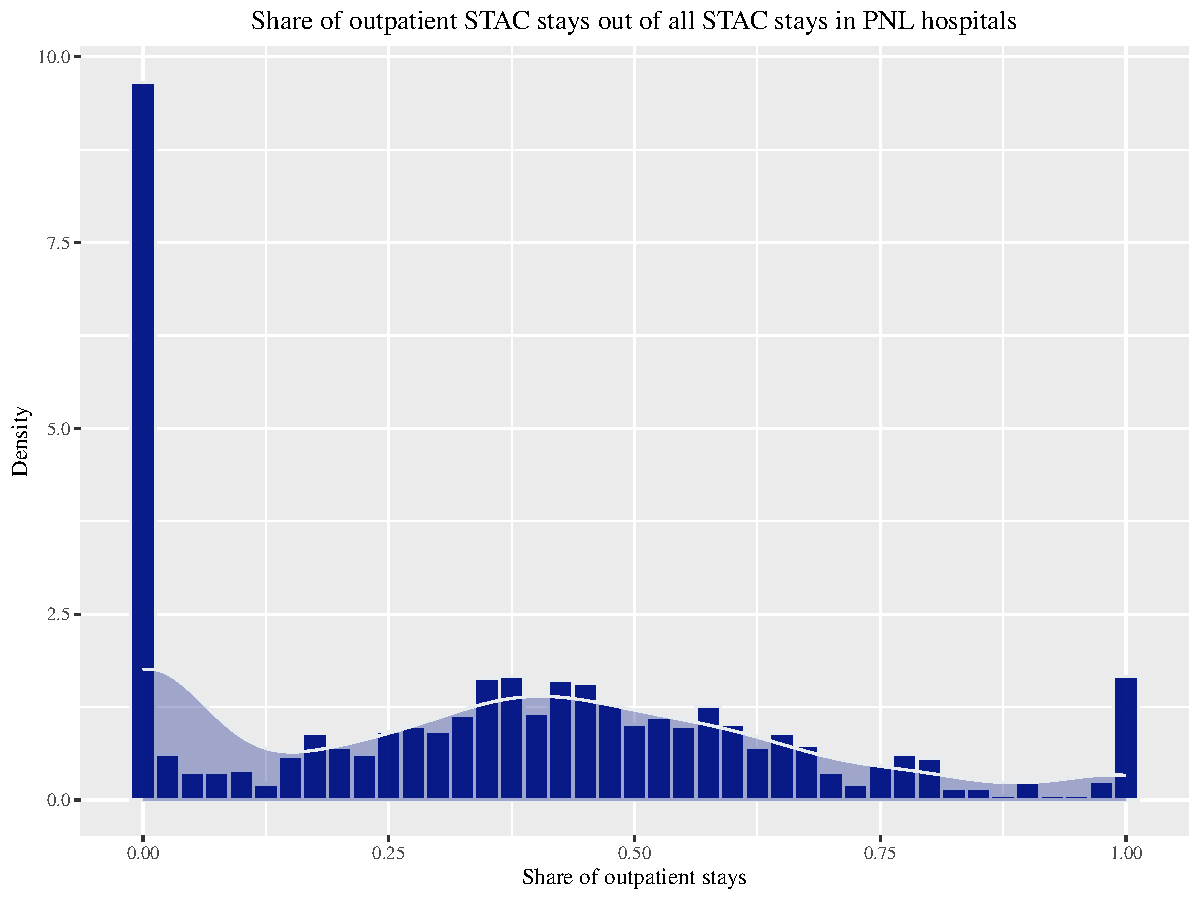
\includegraphics[width=0.8\textwidth]{../../Figures/2016-2022/STAC_share_PNL.pdf}
\end{figure}

\begin{figure}[!htb]
    \centering
    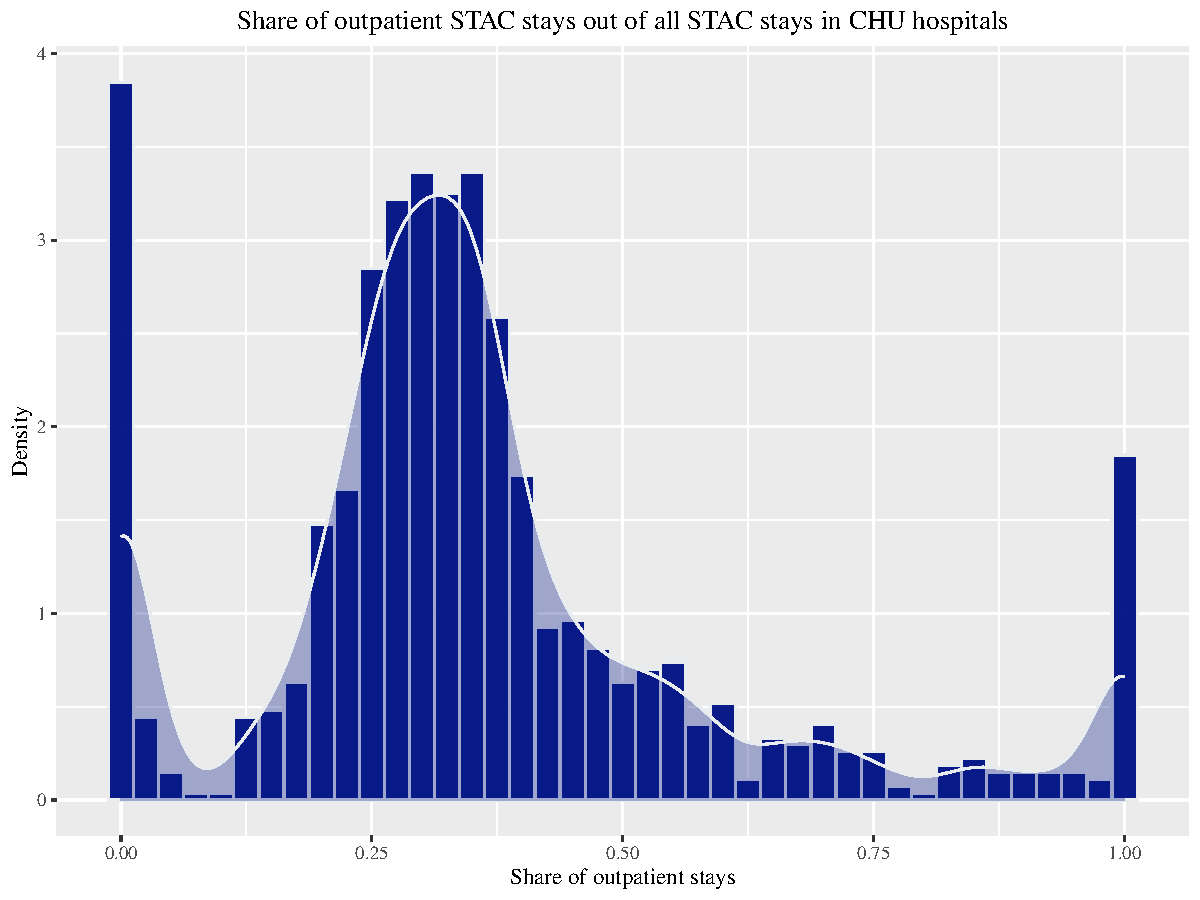
\includegraphics[width=0.8\textwidth]{../../Figures/2016-2022/STAC_share_CHU.pdf}
\end{figure}

\begin{figure}[!htb]
    \centering
    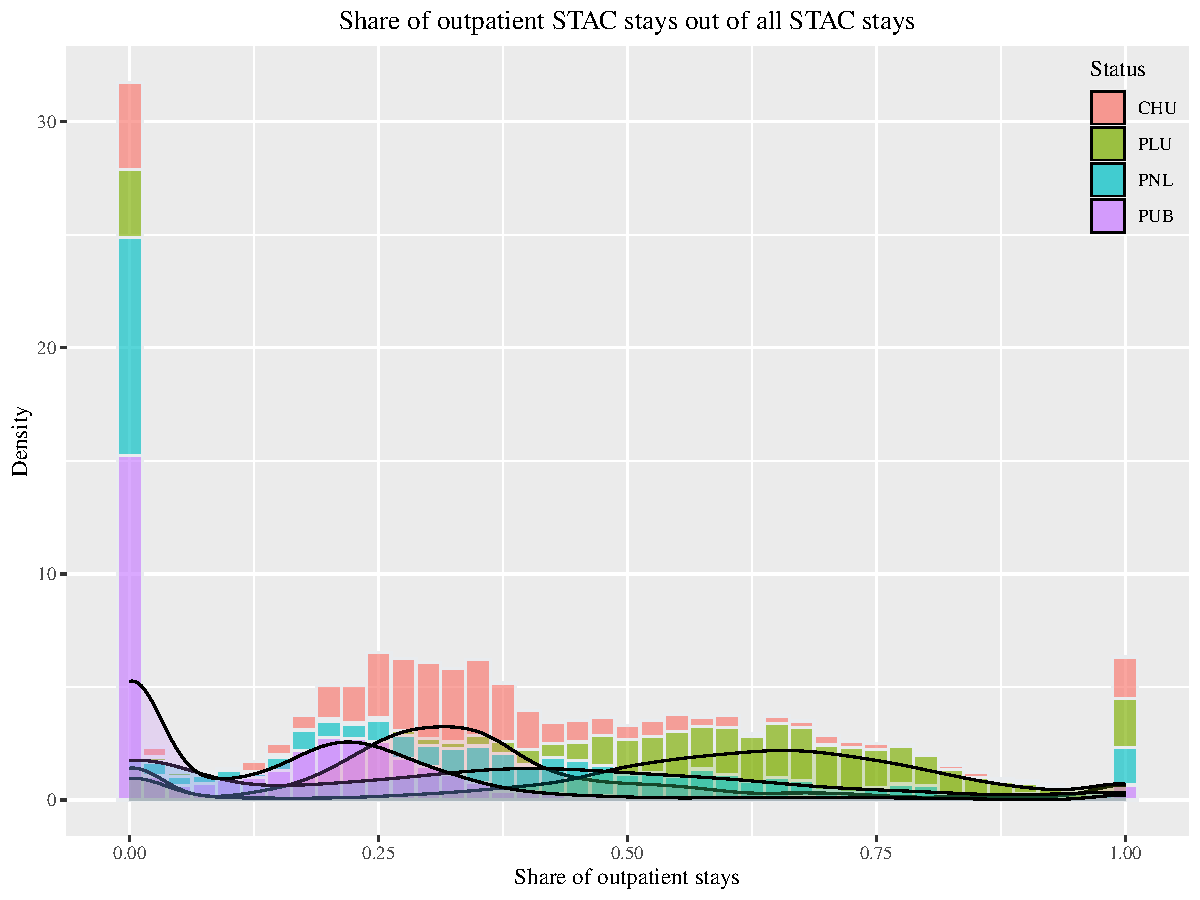
\includegraphics[width=0.8\textwidth]{../../Figures/2016-2022/STAC_share_all.pdf}
\end{figure}
\clearpage
\subsection{Average length of stay}
% latex table generated in R 4.2.1 by xtable 1.8-4 package
% Fri May 10 23:47:28 2024
\begin{table}[ht]
\centering
\begin{tabular}{rlrrrrr}
  \hline
 & STJR\_LABEL & PUB & PLU & PNL & CHU & All \\ 
  \hline
1 & Q1 & 5.12 & 3.13 & 4.22 & 5.05 & 4.05 \\ 
  2 & Q2 & 6.21 & 3.78 & 5.46 & 6.03 & 5.26 \\ 
  3 & Q3 & 11.83 & 4.53 & 10.08 & 8.60 & 8.47 \\ 
  4 & Mean & 8.76 & 4.18 & 7.53 & 7.42 & 6.99 \\ 
  5 & Std\_dev & 5.25 & 2.38 & 5.03 & 4.00 & 4.81 \\ 
  6 & Nobs & 2712.00 & 1926.00 & 715.00 & 584.00 & 5937.00 \\ 
   \hline
\end{tabular}
\end{table}


\begin{figure}[!htb]
    \centering
    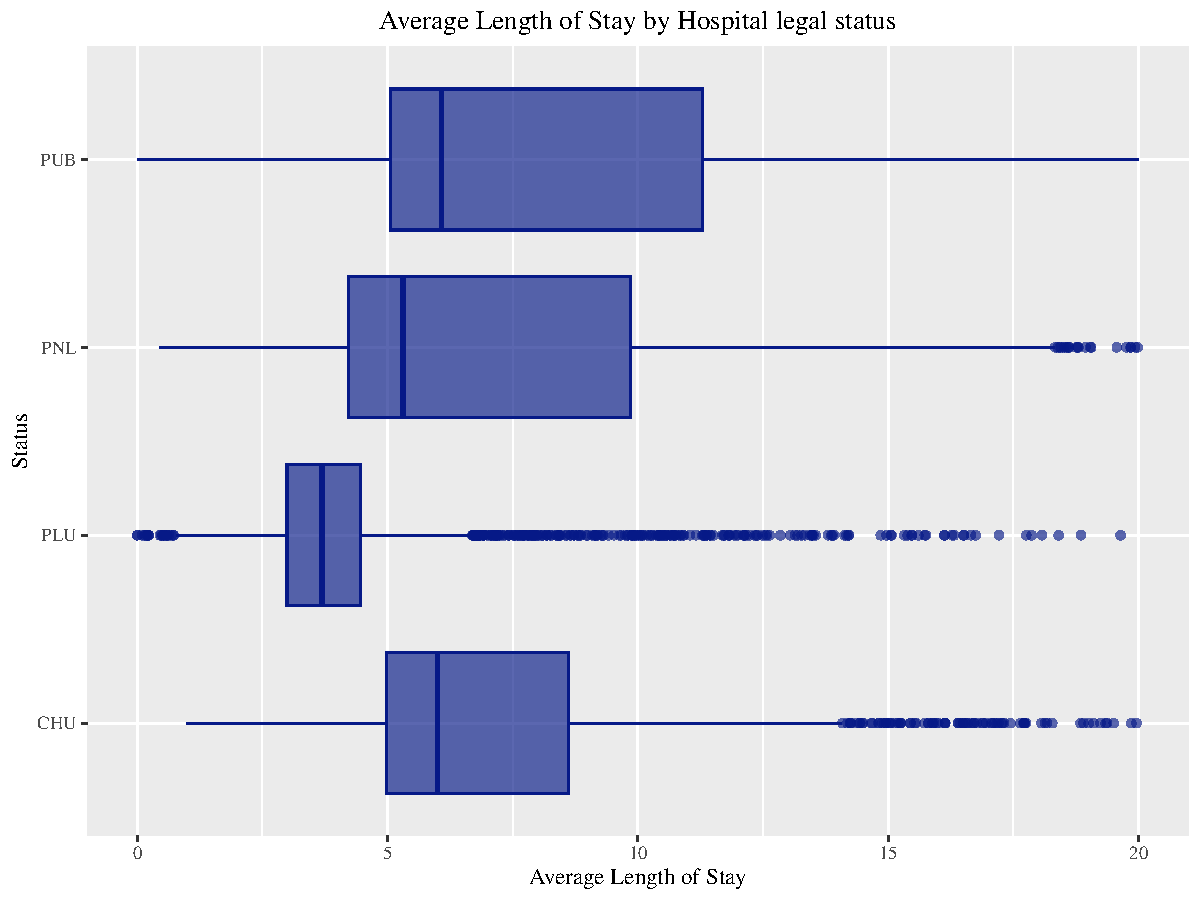
\includegraphics[width=0.8\textwidth]{../../Figures/2016-2022/ALOS.pdf}
\end{figure}
\clearpage
\subsection{Selection of patients}

% latex table generated in R 4.3.1 by xtable 1.8-4 package
% Tue May 14 13:32:48 2024
\begin{table}[ht]
\centering
\begin{tabular}{rlrrrr}
  \hline
 & size & CHU & PLU & PNL & PUB \\ 
  \hline
1 & 1 & 11.85 & 14.89 & 29.51 & 34.51 \\ 
  2 & 2 & 11.72 & 4.57 & 19.02 & 23.70 \\ 
  3 & 3 & 11.73 & 3.56 & 10.85 & 14.75 \\ 
  4 & 4 & 11.44 & 4.59 & 10.50 & 13.96 \\ 
   \hline
\end{tabular}
\caption{Average casemix index by hospital legal status and size of hospital} 
\end{table}


\section{Mixture model}

\subsection{Location mixture}
The model is the following
\begin{equation*}
    y_{it}=\theta_i+\epsilon_{it} \quad \text{where} \quad \epsilon_{it}\sim N(0,1)
\end{equation*}
Thus \begin{equation*}
    \hat{\theta}_i=\frac{1}{T_i}\sum y_{it} \sim N(\theta_i,1/T_i)
\end{equation*}
The likelihood function $L(F|y)$ (optimizing over distribution function $F$ given the observed $y$) is
\begin{equation*}
    \begin{split}
        L(F|y)&=\prod_{i=1}^N\int \prod_{1}^{T_i} \phi(y_{it}-\theta_i)dF(\theta_i)
    \end{split}
\end{equation*}
Instead of focusing on each observation $y_{it}$ we can also focus on the mean $\hat{\theta}_i=\bar{y}_i$.
If we utilize $\hat{\theta}_i-\theta_i \sim N(0,1/T_i)$, we can write the likelihood function as \begin{align*}
    L(F|y) & =\prod_{i=1}^N\int
    \phi((\hat{\theta}_i-\theta_i)\sqrt{T_i})\sqrt(T_i)dF \\
    l(F|y) & =\sum_{i=1}^N\log\int
    \phi((\hat{\theta}_i-\theta_i)\sqrt{T_i})\sqrt(T_i)dF
\end{align*}
Optimizing over all possible function $F$ neccesitates some kind of discrete approximation. The most common one is the grid approximation. We can also use the EM algorithm to optimize the likelihood function.
Let $f_j$ approximate the value of $d F$ on the grid
\begin{equation*}
    \max_f \set{ \sum_{i=1}^N\log g_i \big| g=Af, \sum_j f_j\Delta_j =1, f\ge 0}
\end{equation*}

\begin{remark}
    For a reader not as versed in mathematics as she should be. $A_{i*}f = \sum \sqrt{T_i}\phi((\hat{\theta}_i-\theta_j)\sqrt{T_i})f_j\Delta_j$.
    We use $\sum f_j\Delta_j$ to approximate the integral $\int dF$ as one can imagine.
\end{remark}
This a convex objective function subject to linear equality  and inequality constraints. The EM algorithm is a natural choice to optimize this function. The E-step is to calculate the expectation of the log-likelihood function given the observed data and the current estimate of the parameter. The M-step is to maximize the expectation of the log-likelihood function with respect to the parameter. The algorithm iterates between these two steps until convergence.
Often, the dual formulation of a convex objective is more efficient than the primal.
\begin{equation*}
    \max_f \set{ \sum_{i=1}^N\log (v_i)|A^T v = n 1_p, v\ge 0}
\end{equation*}
\begin{question}
    Derive on your own for practice
\end{question}
\begin{sol}
    We define the multiplier $\mu_1', \mu_2, \lambda'$ for the two equality and one inequality contstraints.
    The dual objective function is \begin{equation*}
        \min_{f,g} \set{-\sum_{i=1}^N\log g_i + \mu_1'(g-Af) + \mu_2(\sum_j f_j\Delta_j-1) - \lambda' f}
    \end{equation*}
    Minimize over each $g_i$ gives the condition \begin{equation*}
        \frac{1}{g_i}=\mu_{1i}
    \end{equation*}
    Minimize over each $f_i$ gives the condition \begin{equation*}
        -(\mu_1'A)_j+\mu_2-\lambda_j=0
    \end{equation*}
    Therefore the objective is \begin{equation*}
        \begin{array}{ll}
                              & \set{\sum \log \mu_{1i} + n - \mu_2 } \\
            \text{subject to} & -\mu_1'A+\mu_2 1_p-\lambda=0          \\
                              & \lambda\ge 0
        \end{array}
    \end{equation*} Thus the dual problem is \begin{equation*}
        \begin{array}{ll}
            \text{maximize}_{\mu_1',\mu_2} & \set{\sum \log \mu_{1i}+n-\mu_2} \\
            \text{subject to}              & \mu_1'A\le \mu_2 1_p             \\
                                           & \mu_1\ge 0
        \end{array}
    \end{equation*}
\end{sol}
\subsection{Scale mixture}
The model is the following:
\begin{equation*}
    y_{it}=\sigma_i\epsilon_{it} \quad \text{where} \quad \epsilon_{it}\sim N(0,1)
\end{equation*}
Similarly \begin{equation*}
    s_i=\hat{\sigma}_i^2=\frac{1}{m_i}\sum_{t=1}^{T_i}y_{it}^2
\end{equation*}
But what's the distribution of $\hat{\sigma}_i$ (which is not so obvious relative to $\hat{\theta}_i$)?
Well, $\frac{\sum y_{it}^2}{\sigma_i^2}$ follows a Gamma distribution with shape parameter $r_i=(T_i)/2$ and scale parameter $s_i=\sigma_i^2/r_i=2\sigma_i^2/T_i$.
\begin{question}
    Why is it gamma distribution?
\end{question}
\begin{sol}
    The sum of k independent standard normal variable  $X$ follows a $\chi^2(k)$ distribution. \\
    The mean of n independent $\chi^2(k)$ distribution variables $K$ follows a gamma distribution $\gamma(nk/2,2/n)$.\\
    The equivalence lies in \href{https://en.wikipedia.org/wiki/Gamma_distribution}{here}: if $X \sim \gamma(v/2, 2)$ (in the shape-scale parametrization), then $X$ is identical to $\chi^2(v)$, the chi-squared distribution with $v$ degrees of freedom. Conversely, if $Q\sim \chi^2(v)$ and c is a positive constant, then $cQ ~ \gamma(v/2, 2c)$.
\end{sol}
\begin{remark}
    The Gamma distribution $\gamma(k, \theta)$ (shape, scale) has the following distribution function \begin{equation*}
        f(x|k,\theta)=\frac{1}{\Gamma(k)\theta^k}x^{k-1}e^{-x/\theta} \quad F(x|k,\theta)=\frac{1}{\Gamma(k)}\gamma(k,x/\theta)
    \end{equation*} where $\Gamma(z)=\int_0^{\infty}t^{z-1}e^{-t}dt$.
\end{remark}
Thus the likelihood function is \begin{align*}
    L(F|y) & =\prod_{i=1}^N\int \gamma(s_i|r_i,\sigma_i)dF(\sigma_i)    \\
    l(F|y) & =\sum_{i=1}^N\log\int \gamma(s_i|r_i,\sigma_i)dF(\sigma_i)
\end{align*}
which we can proceed just as in the location mixture case.
\subsection{Location-scale mixture (independent)}
The model is \begin{equation*}
    y_{it}=\theta_i+\sigma_i\epsilon_{it} \quad \text{where} \quad \epsilon_{it}\sim N(0,1)
\end{equation*}
The sufficient statistics $\hat{\theta}_i$ and $\hat{\sigma}_i$ are \begin{align*}
    \hat{\theta}_i & =\frac{1}{T_i}\sum_{t=1}^{T_i}y_{it} \sim N(\theta_i, \sigma_i^2/T_i)                                       \\
    \hat{\sigma}_i & =\frac{1}{T_i}\sum_{t=1}^{T_i}(y_{it}-\hat{\theta}_i)^2\sim \gamma(s_i | \alpha= r_i, \beta=\sigma_i^2/r_i)\end{align*}
Just as in the previous two cases, we can write the (log) likelihood as \begin{equation*}
    l(G_{\theta},F_{\sigma}|y)=\sum_{i=1}^N\log\int \int \bra{\phi((\hat{\theta}_i-\theta_i)\sqrt{T_i})\sqrt{T_i}} \bra{\gamma(s_i|r_i,\sigma_i)} dG_{\theta}(\theta_i) dF_{\sigma}(\sigma_i)
\end{equation*}
For \textbf{estimation}, we can first solve for $\hat{F}_{\sigma}$ and solve for $\hat{G}_{\theta}$ given $\hat{F}_{\sigma}$. There are two compuatation methods.
\begin{itemize}
    \item Reexpress the Gaussian component as Student's $t$ therefore eliminating the
          dependence on $\sigma_i$.
    \item Iterate between the Gamma and Gaussian component of the likelihood. (Specific
          to this independent prior assumption.)
\end{itemize}
\subsection{Location-scale mixture (general)}
The most general Gaussian location-scale mixture with covariate effects.
\begin{question}
    It seems that in the paper. They assume that the \textbf{TRUE} covariate effect is known by constructing a profile likelihood to estimate the true $\beta$ (covariate effects).w
\end{question}
\begin{remark}
    The $\hat{\beta}$ that maximizes profile likelihood function of the parameter of interests $\beta$ $L_{\hat{\alpha}(\beta)}(\beta)$ follows \begin{enumerate}
        \item $\hat{\alpha}(\beta)=\argmax_{\alpha} L(\alpha,\beta)$
        \item $\hat{\beta}=\argmax_\beta L_{\hat{\alpha}(\beta)}(\beta)$
    \end{enumerate}
    Note that maximizing profile likelihood function to get estimates gives rise to the infamous \textbf{incidental parameter problem} due to the fact that \begin{equation*}
        \hat{\alpha}(\beta)=\frac{1}{T_i}\sum \log(f(\alpha,\beta)) \not\rightarrow \E\bra{\log f(\alpha,\beta)}
    \end{equation*}
\end{remark}
\begin{equation*}
    y_{it}=x_{it}\beta+\theta_i+\sigma_i\epsilon_{it} \quad \text{where} \quad \epsilon_{it}\sim N(0,1)
\end{equation*}
Given a true $\beta$, it is straightforward that \begin{equation*}
    y_{it}|\mu_i,\sigma_i,\beta \sim N(x_{it}\beta+\mu_i,\sigma_i^2)
\end{equation*}
The sufficient statistics for
\begin{itemize}
    \item $\mu_i$: $\bar{y}_i-\bar{x}_i\beta \sim N(\theta_i,\frac{\sigma_i^2}{T_i})$
          \begin{quote}
              contains the between information
          \end{quote}
    \item $\sigma_i^2$: $\frac{1}{T_i-1}\sum_{t=1}^{T_i}(y_{it}-x_{it}\beta-\mu_i)^2$
          It is worth mentioning that \begin{equation*}
              S_i|\mu_i,\sigma_i^2,\beta \sim \gamma(r_i,\sigma_i^2/r_i) \quad \text{where} \quad r_i=(m_i-1)/2
          \end{equation*}
          \begin{quote}
              contains the within information (deviations from the individual means)
          \end{quote}
\end{itemize}
\begin{remark}
    Unlike in the pure scale mixture, we don't know the true location parameter.
    instead of $y_{it}-x_{it}\beta-\theta_i$ as in the scale mixture case, we need to use the sufficient statistics for $\theta_i$, which is $\frac{1}{T}\sum (y_{it}-x_{it}\beta)$. Each $y_{it}-x_{it}\beta-(\bar{y}_i-\bar{x}_i\beta)$ is a normal variable with mean 0 and variance $(1-1/T_i)\sigma_i^2$.\begin{equation*}
        y_{it}-x_{it}\beta-\bar{y}_i+\bar{x}_i\beta \sim N(0,(1-1/T_i)\sigma_i^2)
    \end{equation*}
    If we \textit{may} assume that $z_{it}=y_{it}-x_{it}\beta-\bar{y}_i+\bar{x}_i$ is independent of $z_{it'}$ (which is not, the covariance is $\frac{1}{T(T-1)}\sigma_i^2$), then the sufficient statistics \begin{equation*}
        S_i'=\sum (\frac{1}{\sqrt{T_i-1}}z_{it})^2 \underbrace{\sim}_{\text{if we may assume}} \sum \frac{\sigma_i^2}{{T_i}}Z_{it}^2 \sim \frac{\sigma_i^2}{T_i}\chi^2(T_i) \sim \gamma(\frac{T_i-1}{2},\frac{2\sigma^2}{T_i})
    \end{equation*} where $Z_{it}\sim N(0,1)$ and are iid.

\end{remark}
\begin{question}
    Why is the derived distribution of $S_i'$ different from $\gamma(\frac{T_i-1}{2},\frac{2\sigma_i^2}{T_i-1})$?
\end{question}
\begin{remark}
    The orthogonality between the within and between information no longer holds here. (Why does it hold in the classical Gaussian panel data?)
\end{remark}
The likelihood function is \begin{equation*}
    \begin{split}
        l(\beta, h(\theta,\sigma)|y)&=\prod_{i=1}^N g_i(\beta,\theta_i,\sigma_i|y_{i1},\ldots,y_{iT})\\
        &=\prod_{i=1}^N\int \int \prod \frac{1}{\sigma} \phi(\frac{y_{it}-x_{it}\beta-\theta_i}{\sigma}) h(\theta,\sigma)d\theta d\sigma\\
        & =K \prod_{i=1}^N\int S_i^{1-r_i}\int\int \frac{1}{\sigma} \phi(\frac{\bar{y}_{i}-\bar{x}_{i}\beta-\theta_i}{\sigma})\frac{e^{-R_i}R_i^{r_i}}{S_i\Gamma(r_i)}h(\theta, \sigma)d\theta d\sigma
    \end{split}
\end{equation*}
where \begin{equation*}
    \begin{array}{ll}
        R_i=\frac{r_iS_i}{\sigma_i^2} & K=\prod_{i=1}^N\ \pa{\frac{\Gamma(r_i)}{r_i^{r_i}}(\frac{1}{\sqrt{2\pi}})^{T_i-1}}
    \end{array}
\end{equation*}

\begin{question}
    The true $\beta$ is unknown. Therefore, we can not condition on it. How about the so called profile likelihood? How to compare it with the \textit{FORBIDDEN} approach of getting fixed effect estimates from the WG estimation? Since the $\theta_i$ is regarded as \textit{NUISANCE} parameters in the WG estimation, how low the status is...! Poor $\theta_i$!
\end{question}

\begin{example}
    Consider a simple model where \begin{equation*}
        y_{it}=\alpha_i f(x_{it};\beta)\epsilon_{it}
    \end{equation*}
    and $\epsilon|\alpha_i,x_{it}\sim \calp(1)$ Then we have \begin{equation*}
        y_{it} | \alpha_i,\pa{m_{it}= f(x_{it};\beta)}\sim \calp(\alpha_i m_{it})
    \end{equation*}
\end{example}


% 
\subsection{Estimation of mixture density}
\paragraph{Dependent of location and scale}
\begin{figure}
    \centering
    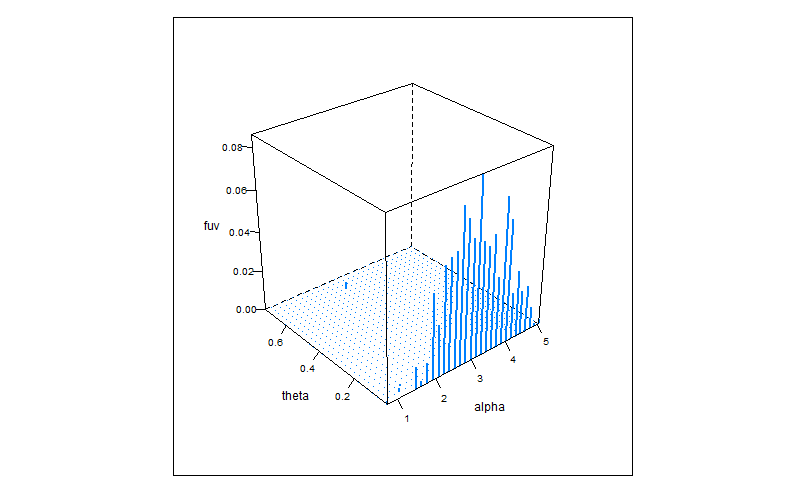
\includegraphics[width=0.8\textwidth]{../../Figures/2016-2022/WGLVmix.png}
\end{figure}

\paragraph{Independent location and scale}
\begin{figure}
    \centering
    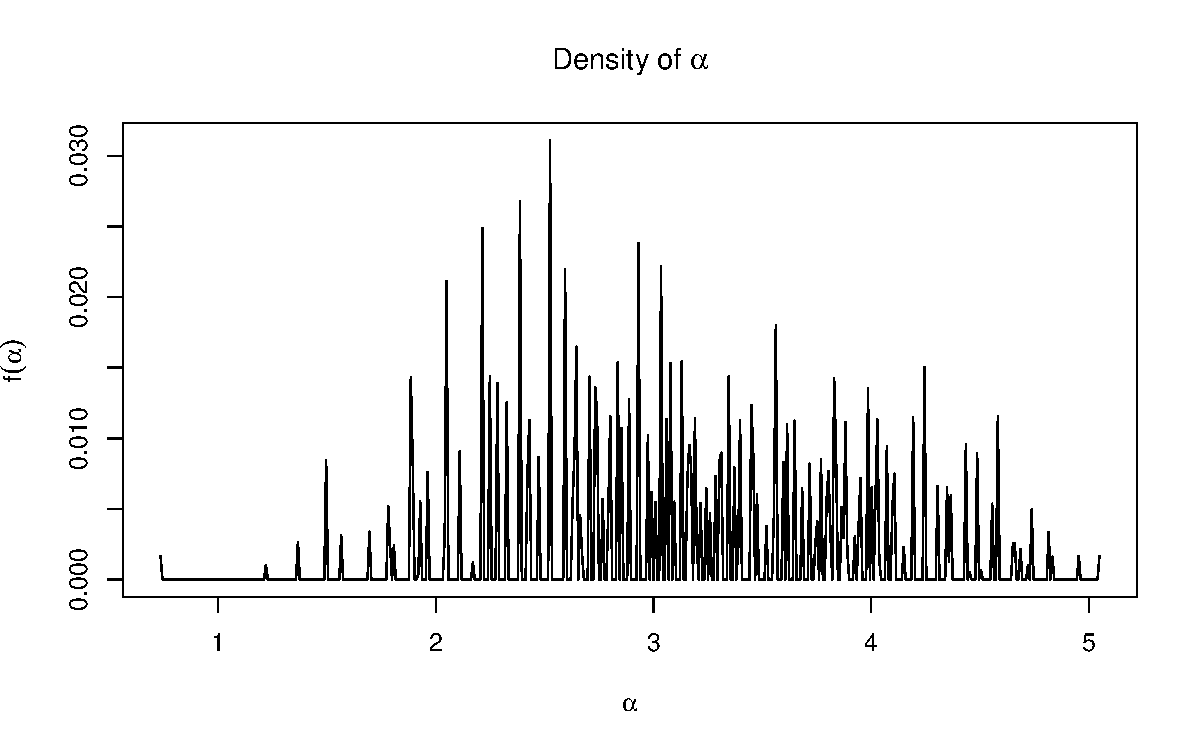
\includegraphics[width=0.8\textwidth]{../../Figures/2016-2022/WTLVmix_u.pdf}
    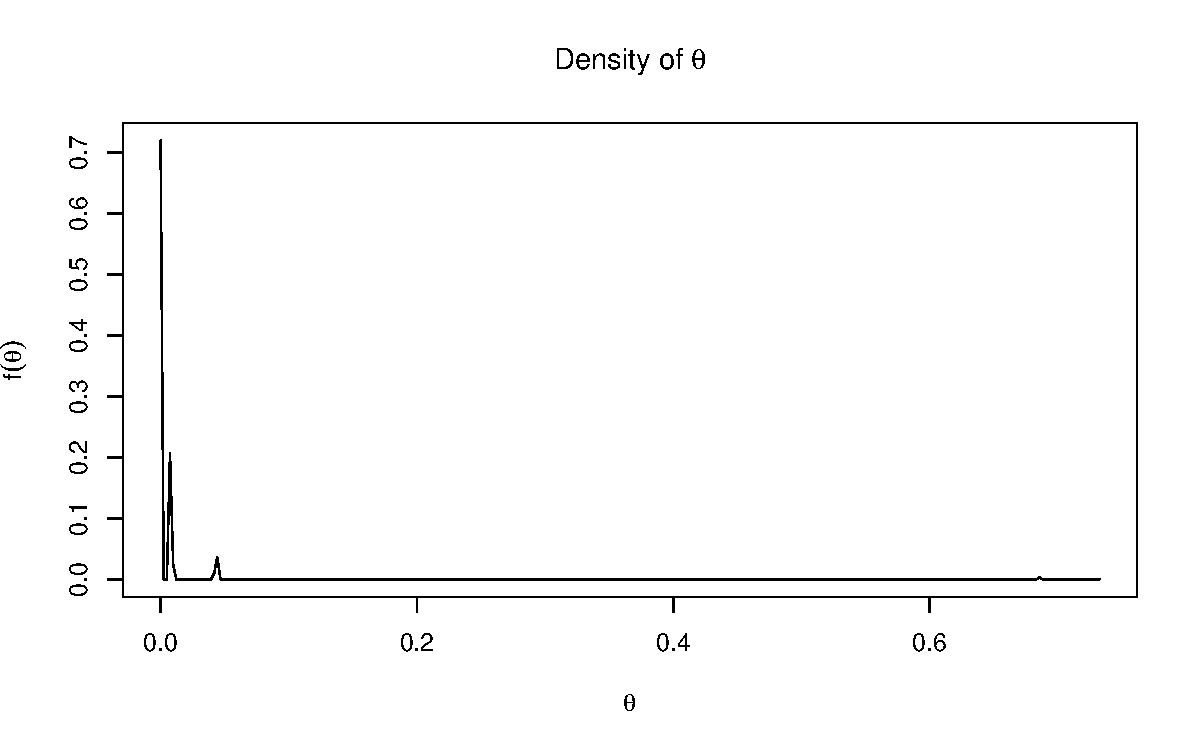
\includegraphics[width=0.8\textwidth]{../../Figures/2016-2022/WTLVmix_v.pdf}
\end{figure}


\section{Ranking and Selection}



\end{document}
